%Requires texlive-latex-recommended and texlive-fonts-recommended packages (Debian, Ubuntu).
\documentclass[a4paper,oneside,openany,12pt]{memoir}
\usepackage[T1]{fontenc} % To get different font encoding, thus allow \guillemotright.
% Undo bad "side effects" of T1 font encoding (ugly font && chapters in small caps).
% Note that it's now not shown in small caps simply because the selected font does not support it.
\usepackage{lmodern}
\usepackage{graphicx} % For images
\graphicspath{{../gfx/}}
%\usepackage[english]{babel} % For correct word hyphenating.
\usepackage{color}    % For colored links and boxes.
\usepackage[dvipsnames]{xcolor}
\definecolor{LOVDdark}{HTML}{224488}
\definecolor{LOVDlight}{HTML}{F0F3FF}
\usepackage{float}    % For custom floats (the info boxes).
\usepackage{wrapfig}  % For floating boxes meant for small notes.
% When loaded before float, doesn't work.
% For figures, maybe not do an frame but a box without border and with background color?
\usepackage[format=hang,font=footnotesize,labelfont=bf,skip=5pt]{caption} % To format captions.
\usepackage{hyperref} % For URLs.
\usepackage{tikz}
\usepackage{xr}

% Include all of this in a separate file!
\newcommand{\HRule}{\rule{\linewidth}{1mm}} % Doet height (zie style) hetzelfde?
\newcommand{\institute}[1]{\gdef\inst{#1}}  % Beamer supplies \institute. We want that, too.
\newcommand{\inst}{}                        % Beamer supplies \institute. We want that, too.
\newcommand{\funding}[1]{\gdef\fund{#1}}    % Provide funding line.
\newcommand{\fund}{}                        % Provide funding line.
\newcommand{\setcreativecommons}[1]{\gdef\creativecommons{#1}}	% Provide creative commons line.
\newcommand{\creativecommons}{}                       			 		% Provide creative commons line.
\newcommand{\setLOVDversion}[1]{\gdef\LOVDversion{#1}} % Provide the current LOVD version.
\newcommand{\LOVDversion}{}                            % Provide the current LOVD version.
\newcommand{\setpointercolor}[1]{\gdef\pointercolor{#1}}%
\newcommand{\pointercolor}{}  													%
\newcommand{\setpointerwidth}[1]{\gdef\pointerwidth{#1}}%
\newcommand{\pointerwidth}{}  													%
\newcommand{\setgrid}[1]{\gdef\drawgrid{#1}}						% Used for drawing a grid over a figure
\newcommand{\drawgrid}{} 																%
\newcommand{\setmanualversion}[1]{\gdef\manualversion{#1}} 	% Provide the current manual version.
\newcommand{\manualversion}{}                            		% Provide the current manual version.

\setlrmarginsandblock{2cm}{2cm}{*} % LEFT-RIGHT
\setulmarginsandblock{2cm}{2cm}{*} % TOP-BOTTOM
\checkandfixthelayout % Without this, nothing works. Took me ages before I found out.
\fixpdflayout % Not sure if we need this, but it was recommended someplace.



%%%%% PAGE HEADERS AND FOOTERS %%%%%
\makepagestyle{LOVD}

% Because we don't have odd or even pages, we only need to define odd pages.
\makeoddhead{LOVD}{\normalfont\leftmark}{}{\normalfont\rightmark}
\makeheadrule{LOVD}{\textwidth}{\normalrulethickness}
\makeoddfoot{LOVD}{}{\normalfont\thepage}{}
\makefootrule{LOVD}{\textwidth}{\normalrulethickness}{\footruleskip}

% Style "plain" is called from chapters. We want chapters to have a footer as well.
\makeoddfoot{plain}{}{\normalfont\thepage}{}
\makefootrule{plain}{\textwidth}{\normalrulethickness}{\footruleskip}

% Additional changes:
\makepsmarks{LOVD}{%
  \nouppercaseheads

  \createmark{chapter}{left}{shownumber}{}{.\space} % (\leftmark) number, followed by a . and a space.
  \createmark{section}{right}{nonumber}{}{.\space} % (\rightmark) no number, (useless: followed by a . and a space).
  % Change "shownumber" to "nonumber" if you don't want the chapter/section number displayed at the header.
}
% Activate your new pagestyle
\pagestyle{LOVD}



%%%%% TITLE PAGE FORMAT %%%%%
\setlength{\droptitle}{-3cm} % Moves the title (logo, title, authors etc) 3cm up.
\pretitle{
  \begin{center}
  	
\includegraphics[width=16cm]{logo.jpg}
    \vskip 1.5cm
   	
\includegraphics[width=3cm]{hgvs.png} \hspace{1.5cm}
		
\includegraphics[width=3cm]{human_variome.png} \hspace{1.5cm}
    
\includegraphics[width=3cm]{gen2phen.jpg}
    \vskip 3cm
    \HRule\par\HUGE\bfseries\sffamily} %% Need proper font!
\posttitle{\par\HRule\end{center}\vskip 1cm}
\preauthor{\flushright \vskip12em}
\postauthor{\par\inst\par\vskip 5mm}
\predate{\hfill  Last updated: }
\postdate{\par\vskip 5mm\hfill Version: \manualversion 
	\par\hfill Based on LOVD: \LOVDversion 
	\par\clearpage \hfill \vskip50em \small \noindent \fund \creativecommons} 



%%%%% CHAPTER STYLE (CHAPTER HEADS) %%%%%
\makechapterstyle{LOVD}{%
  \setlength\beforechapskip{10pt} % A small distance just above the new Chapter title.
  \setlength\afterchapskip{20pt} % A small distance between the Chapter title and the text.
  \renewcommand{\chapterheadstart}{\vspace*{\beforechapskip}\hrule height 2pt \medskip} % Nice ruler above the Capter title.
  \renewcommand{\chapnamefont}{\normalfont\large\scshape} % CHAPTER
  \renewcommand{\chapnumfont}{\normalfont\huge\bfseries\scshape} % 1
  \renewcommand{\chaptitlefont}{\normalfont\huge\bfseries\scshape} % e.g. "Introduction"
  \renewcommand{\printchaptername}{} % Empty text instead of "Chapter".
                  \renewcommand{\chapternamenum}{ } % Weet niet wat dit anders doet.
                  \renewcommand{\printchapternum}{\chapnumfont \thechapter} % Weet niet wat dit anders doet.
  \renewcommand{\afterchapternum}{. } % Just a dot after the Chapter number, no new line.
  \renewcommand{\afterchaptertitle}{\par\nobreak\medskip\hrule\vskip\afterchapskip} % Nice ruler below the Capter title.
}
\chapterstyle{LOVD}



%%%%% LINK CONFIGURATION %%%%%
\definecolor{linkblue}{rgb}{0.1, 0, 1}
\hypersetup{
  colorlinks,
  citecolor=linkblue,
  filecolor=linkblue,
  linkcolor=linkblue,
  urlcolor=linkblue
}



%%%%% INFOTABLE AND WARNTABLE DEFINITIONS %%%%%
\newsavebox{\infobox}
\newlength{\infoboxlength}
\newlength{\infoboxinnerlength}
\setlength{\infoboxlength}{\textwidth}
\addtolength{\infoboxlength}{-2\fboxsep}
\addtolength{\infoboxlength}{-2\fboxrule}
\addtolength{\infoboxlength}{-1.7cm} % Manually configured value making sure the whole box doesn't exceed the line width.
\setlength{\infoboxinnerlength}{\infoboxlength}
\addtolength{\infoboxinnerlength}{-5pt} % Manually configured value making sure the text doesn't get too near the right border.

%%%%%% DEFINITIONS FOR \FBOX %%%%%%%
\setlength{\fboxsep}{2pt}%
\setlength{\fboxrule}{2pt}%

\newenvironment{infotable}
  {\begin{lrbox}{\infobox}%
    \begin{minipage}[t]{1.5cm}
      \centering
      \vspace{0pt}
      
\includegraphics[width=1cm,height=1cm]{lovd_information.png}
    \end{minipage}
   \begin{minipage}[t]{\infoboxlength}\vspace{5pt}\begin{minipage}{\infoboxinnerlength}}
  {\vspace{6pt}\end{minipage}\end{minipage}\end{lrbox}%
   \begin{center}
   \fcolorbox{black}{LOVDlight}{\usebox{\infobox}}
   \end{center}}

\newenvironment{warntable}
  {\begin{lrbox}{\infobox}%
    \begin{minipage}[t]{1.5cm}
      \centering
      \vspace{0pt}
      
\includegraphics[width=1cm,height=1cm]{lovd_warning.png}
    \end{minipage}
   \begin{minipage}[t]{\infoboxlength}\vspace{5pt}\begin{minipage}{\infoboxinnerlength}}
  {\vspace{6pt}\end{minipage}\end{minipage}\end{lrbox}%
   \begin{center}
   \fcolorbox{black}{LOVDlight}{\usebox{\infobox}}
   \end{center}}



%%%%% CONFIGURE LEFTBAR (FRAMED PACKAGE) %%%%%
% Taken and adapted from http://tex.stackexchange.com/questions/22526/regarding-the-leftbar-environment
% (thanks, xport & Martin Scharrer)
% I still don't like the space between the bar and the colorbox (can be removed by taking out the \hspace), but
% I want that space *inside* the colorbox.
\renewenvironment{leftbar}[1][\hsize]
{%
    \def\FrameCommand
    {%
        {\color{LOVDdark}\vrule width 3pt \hspace{5pt}}%
        \colorbox{LOVDlight}%
    }%
    \MakeFramed{\hsize#1\advance\hsize-\width\FrameRestore}%
}
{\endMakeFramed}



%%%%% CONFIGURE IMAGES %%%%%
\definecolor{shadecolor}{RGB}{240, 243, 255} %F0F3FF
\setgrid{\draw[help lines,xstep=.05,ystep=.05] (0,0) grid (1,1);
	\foreach \x in {0,1,...,9} { \node [anchor=north] at (\x/10,0) {0.\x}; }
	\foreach \y in {0,1,...,9} { \node [anchor=east] at (0,\y/10) {0.\y}; }}
%\newlength{\imagewidth}
%\setlength{\imagewidth}{\textwidth}
%\addtolength{\imagewidth}{-2\FrameSep}
%\addtolength{\imagewidth}{-2\FrameRule}

%%%%% SETTINGS FOR THE TITLE PAGE %%%%%
\institute{Leiden University Medical Center}
\funding{LOVD has received funding from the European Community's Seventh Framework Programme\\
  (FP7/2007-2013) under grant agreement no 200754 - the GEN2PHEN project.}
\setcreativecommons{
	\begin{flushleft}

	
\includegraphics[width=3cm]{cc88x31.png} 
	\vskip1em
	\noindent This work is licensed under the Creative Commons
	Attribution-ShareAlike 4.0 International License. 
	To view a copy of this license, visit http://creativecommons.org/licenses/by-sa/4.0/
 	or send a letter to: Creative Commons, PO Box 1866, Mountain View, CA 94042, USA.
\end{flushleft}}


%%%%% Cross-referencing between different files %%%%%
\externaldocument[create_gene_]{Create_a_gene_variant_database}
\externaldocument[curate_gene_]{Curate_a_gene_variant_database}

%%%%%%%%%%%%%%%%%%%%%%%%%%%%%%%%%%%%%%%%%% NEW MAXIMUM LINE LENGTH (120 char) %%%%%%%%%%%%%%%%%%%%%%%%%%%%%%%%%%%%%%%%%%


%%%%%%%%%%%%%%%%%%%%%%%%%%%%%%%%%%%%%%%%%% NEW MAXIMUM LINE LENGTH (120 char) %%%%%%%%%%%%%%%%%%%%%%%%%%%%%%%%%%%%%%%%%%

%%%%% SETTINGS FOR THE TITLE PAGE %%%%%
\setLOVDversion{3.0-14}
\setmanualversion{1.04}
\title{LOVD3 Course \\\vskip 0.2cm Curate gene variant database (LSDB) \\\vskip 0.2cm Build \LOVDversion}
\author{Daan Asscheman \\ Ivo F.A.C. Fokkema}
\setpointercolor{red}
\setpointerwidth{9pt}






\begin{document}

\begin{titlingpage} % We don't want the front to count as page 1.
\maketitle
\end{titlingpage}





\hypertarget{toc}{}
\tableofcontents










\chapter{Editing a curator account}
The objective of this chapter is:
\begin{enumerate}
	\item 
	Edit some basic information of the curator user account.
\end{enumerate}
To start this chapter:
\begin{itemize}
	\item 
	Go to \url{http://courses.lovd.nl/LOVD3/} and select the directory corresponding to the number assigned to
	 you.
	\item
	Log in as Manager (with for every one the same username: manager, password: \newline manager1).
\end{itemize}

\begin{figure}[ht]
  \begin{shaded}
		\frame{
			\begin{tikzpicture}
		  	\node[anchor=south west,inner sep=0] (image) at (0,0) {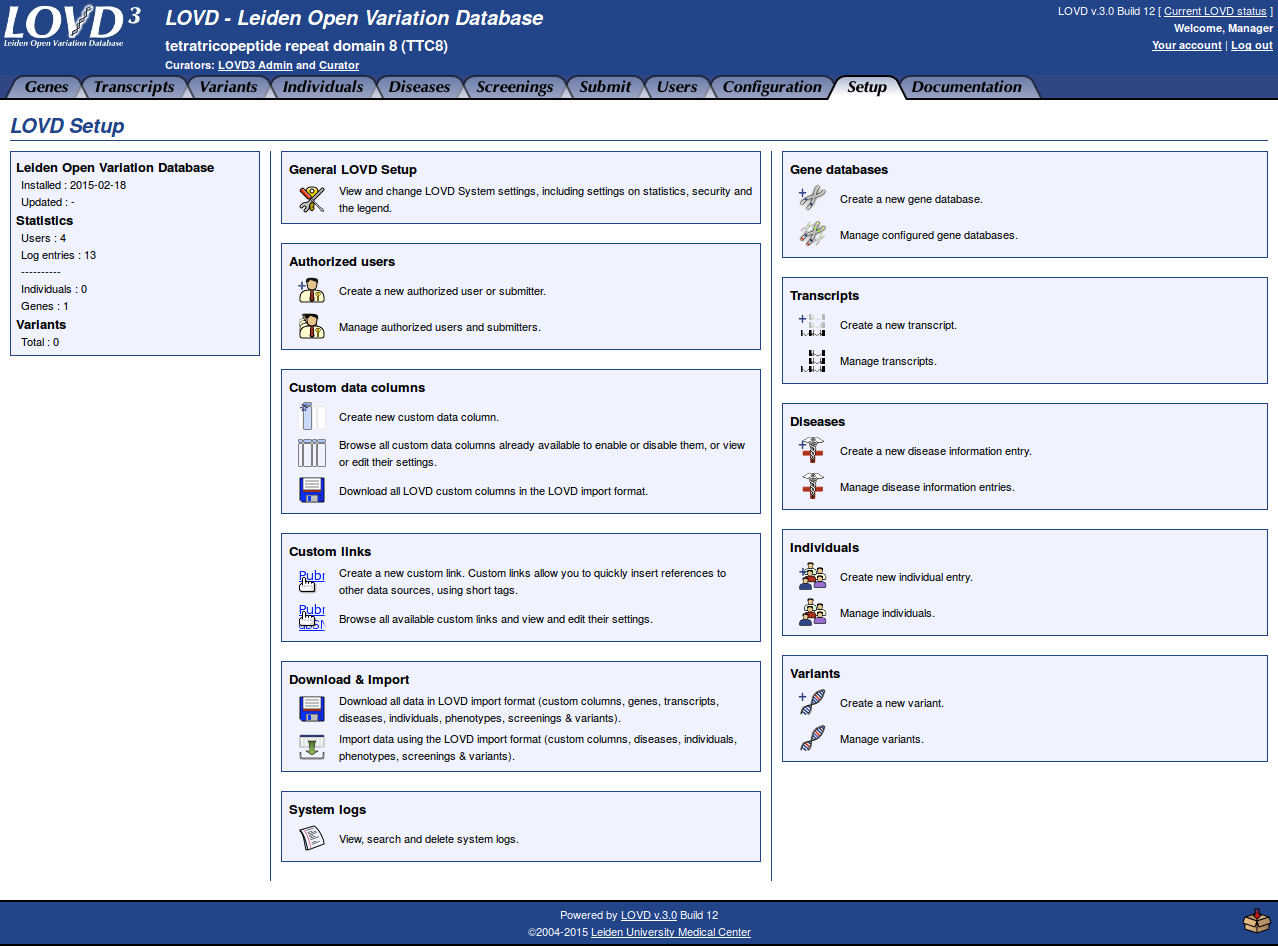
\includegraphics[width=\linewidth]
		   	 {/curate_gene/edit_curator_I.png}};
		  	\begin{scope}[x={(image.south east)},y={(image.north west)}]
		      \draw[red,ultra thick,rounded corners] (0.645,0.89) rectangle (0.71,0.925);
					\draw[<-, >=latex, \pointercolor, line width=\pointerwidth] (0.71,0.9075) to node[black]{A} (0.81,0.9075);
			    \draw[red,ultra thick,rounded corners] (0.22,0.63) rectangle (0.45,0.68);
					\draw[<-, >=latex, \pointercolor, line width=\pointerwidth] (0.45,0.655) to node[black]{B} (0.55,0.655);
			    \draw[red,ultra thick,rounded corners] (0.5,0.89) rectangle (0.56,0.925);
					\draw[<-, >=latex, \pointercolor, line width=\pointerwidth] (0.5,0.9075) to node[black]{C} (0.4,0.9075);
					%\drawgrid %help grid when positioning the boxes and pointers
		  	\end{scope}
			\end{tikzpicture}}
	  \caption{If you want to edit a user account you have to go to ``View user accounts'' and select a user.
		You can do that from the Setup area (A), click the ``Manage authorized users and submitters.'' link listed under
			``Authorized users''(B). \newline
		Alternative: Go directly to ``View users accounts'' via the Users menu tab (C).}
		\label{fig:edit_curator_I}
  \end{shaded}
\end{figure}

\begin{figure}[ht]
  \begin{shaded}
		\frame{
			\begin{tikzpicture}
		  	\node[anchor=south west,inner sep=0] (image) at (0,0) {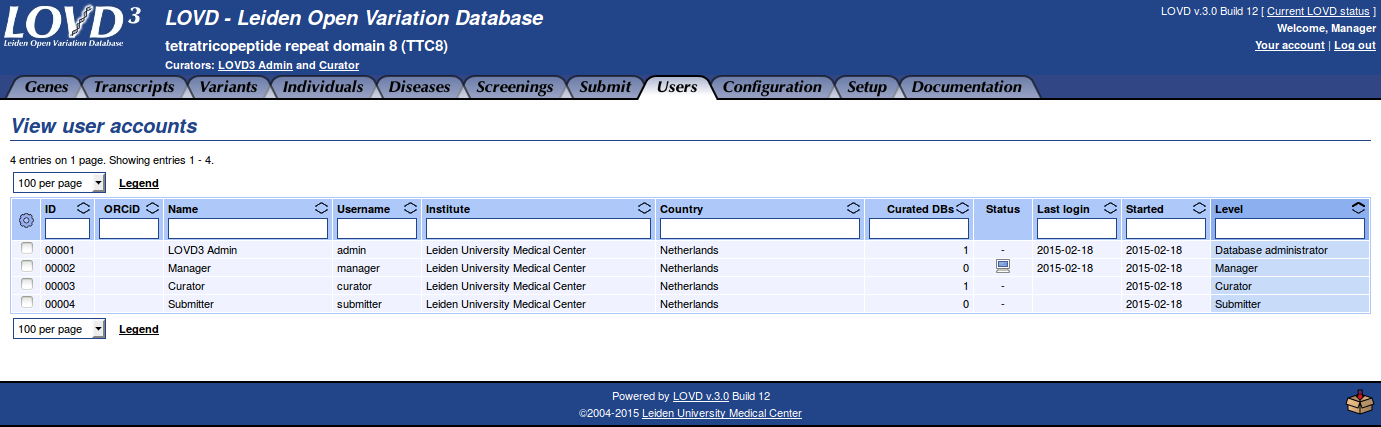
\includegraphics[width=\linewidth]
		   	 {/curate_gene/edit_curator_II.png}};
		  	\begin{scope}[x={(image.south east)},y={(image.north west)}]
		      \draw[red,ultra thick,rounded corners] (0.01,0.31) rectangle (0.55,0.36);
					\draw[<-, >=latex, \pointercolor, line width=\pointerwidth] (0.55,0.335) to node[black]{} (0.65,0.335);
					%\drawgrid %help grid when positioning the boxes and pointers
		  	\end{scope}
			\end{tikzpicture}}
	  \caption{Select the user you want to edit, in this example, the curator.}
		\label{fig:edit_curator_II}
  \end{shaded}
\end{figure}

\begin{figure}[ht]
  \begin{shaded}
		\frame{
			\begin{tikzpicture}
		  	\node[anchor=south west,inner sep=0] (image) at (0,0) {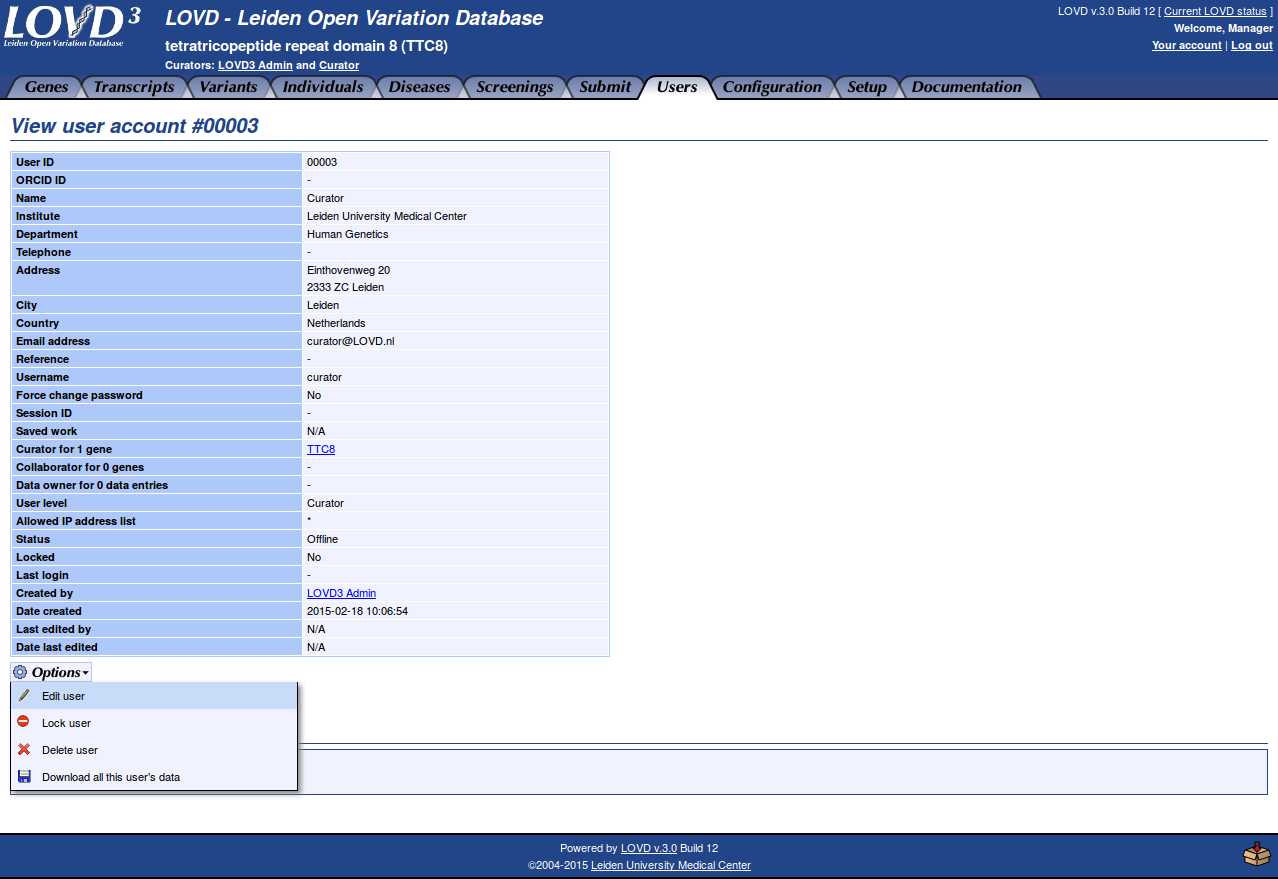
\includegraphics[width=\linewidth]
		   	 {/curate_gene/edit_curator_III.png}};
		  	\begin{scope}[x={(image.south east)},y={(image.north west)}]
		      \draw[red,ultra thick,rounded corners] (0.005,0.195) rectangle (0.11,0.225);
					\draw[<-, >=latex, \pointercolor, line width=\pointerwidth] (0.11,0.21) to node[black]{} (0.21,0.21);
					%\drawgrid %help grid when positioning the boxes and pointers
		  	\end{scope}
			\end{tikzpicture}}
	 		\caption{Click the Options drop down menu and select ``Edit user''.}
		\label{fig:edit_curator_III}
  \end{shaded}
\end{figure}

\begin{figure}[ht]
  \begin{shaded}
		\frame{
			\begin{tikzpicture}
		  	\node[anchor=south west,inner sep=0] (image) at (0,0) {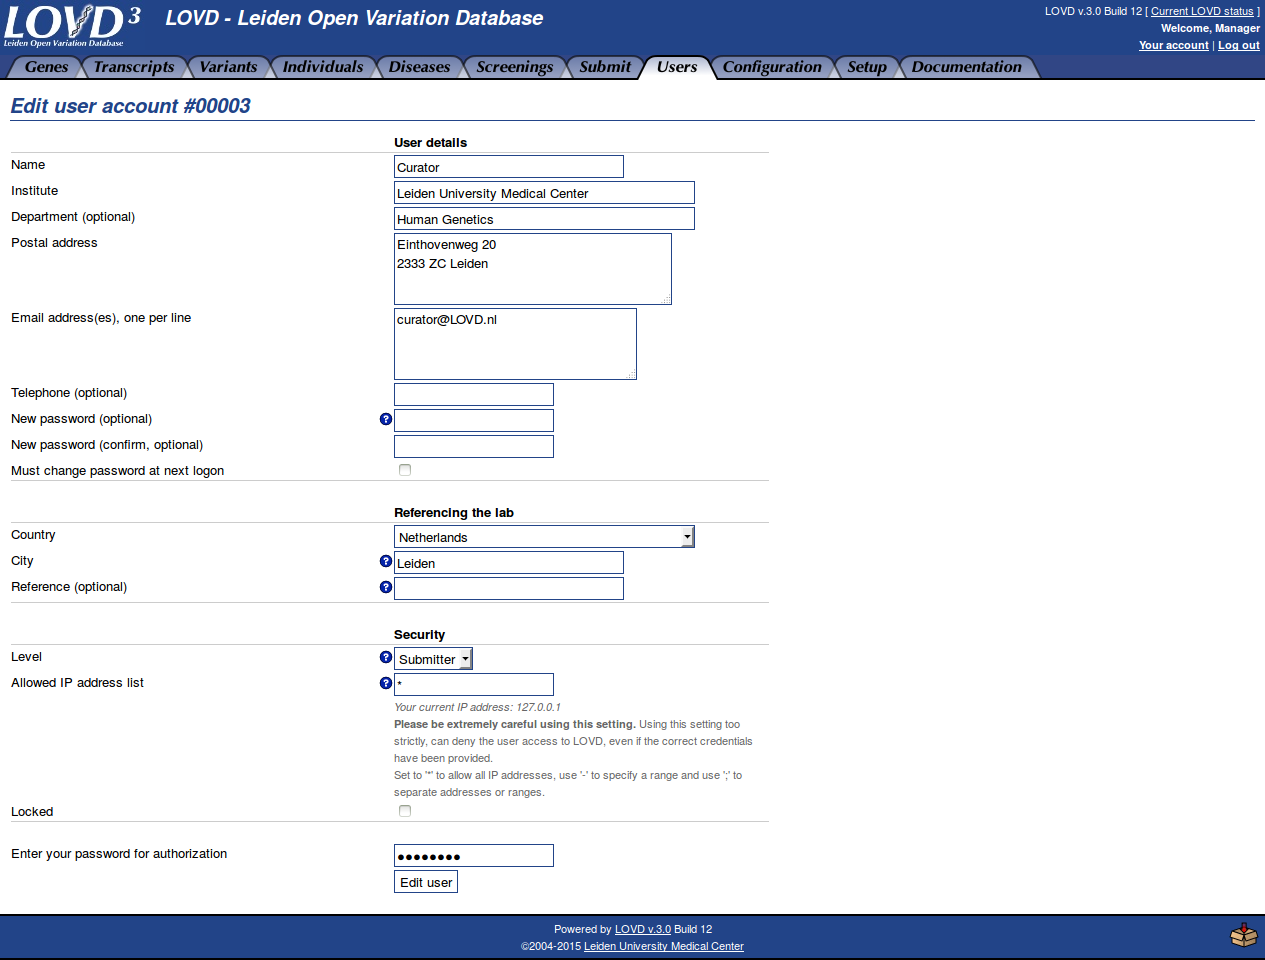
\includegraphics[width=\linewidth]
				{/curate_gene/edit_curator_IV.png}};
		  	\begin{scope}[x={(image.south east)},y={(image.north west)}]
		      \draw[red,ultra thick,rounded corners] (0.305,0.81) rectangle (0.45,0.84);
					\draw[<-, >=latex, \pointercolor, line width=\pointerwidth] (0.45,0.825) to node[black]{A} (0.55,0.825);
		      \draw[red,ultra thick,rounded corners] (0.305,0.60) rectangle (0.51,0.685);
					\draw[<-, >=latex, \pointercolor, line width=\pointerwidth] (0.51,0.6425) to node[black]{B} (0.61,0.6425);
					\draw[red,ultra thick,rounded corners] (0.305,0.52) rectangle (0.44,0.58);
					\draw[<-, >=latex, \pointercolor, line width=\pointerwidth] (0.44,0.55) to node[black]{C} (0.54,0.55);
					\draw[-, >=latex, \pointercolor, line width=0.2*\pointerwidth] (0.307,0.52) to node[black]{} (0.44,0.58);	
					\draw[-, >=latex, \pointercolor, line width=0.2*\pointerwidth] (0.307,0.58) to node[black]{} (0.44,0.52);;
		      \draw[red,ultra thick,rounded corners] (0.305,0.065) rectangle (0.45,0.135);
					\draw[<-, >=latex, \pointercolor, line width=\pointerwidth] (0.45,0.1) to node[black]{D} (0.55,0.1);
		      \draw[red,ultra thick,rounded corners] (0.96,0.93) rectangle (0.998,0.97);
					\draw[<-, >=latex, \pointercolor, line width=\pointerwidth] (0.96,0.93) to node[black]{E} (0.89,0.8);
					%\drawgrid %help grid when positioning the boxes and pointer
		  	\end{scope}
			\end{tikzpicture}}
	  \caption{Insert your name, in place of ``Curator'' (A).\newline
	  Change the e-mail address to your address (so you can receive notifications of new submissions) (B).
		For the course: \textbf{do not change the password} (C).\newline
		Confirm changes with the Manager password, submit the form (D) and log out (E).}
		\label{fig:edit_curator_IV}
  \end{shaded}
\end{figure}



\hypertarget{chap:edit_gene_database}{}
\chapter{Editing a gene database}
\label{chap:edit_gene_database}
The objectives of this chapter are:
\begin{enumerate}
	\item 
	Inspect form ``Edit gene information entry''.
	\item 
	Create and add a disease to a gene via the ``Edit gene information entry'' form.
\end{enumerate}
To start this chapter:
\begin{itemize}
	\item
	Log in as Curator (username: curator, password: curator1).
\end{itemize}

\begin{figure}[ht]
  \begin{shaded}
		\frame{
			\begin{tikzpicture}
		  	\node[anchor=south west,inner sep=0] (image) at (0,0) {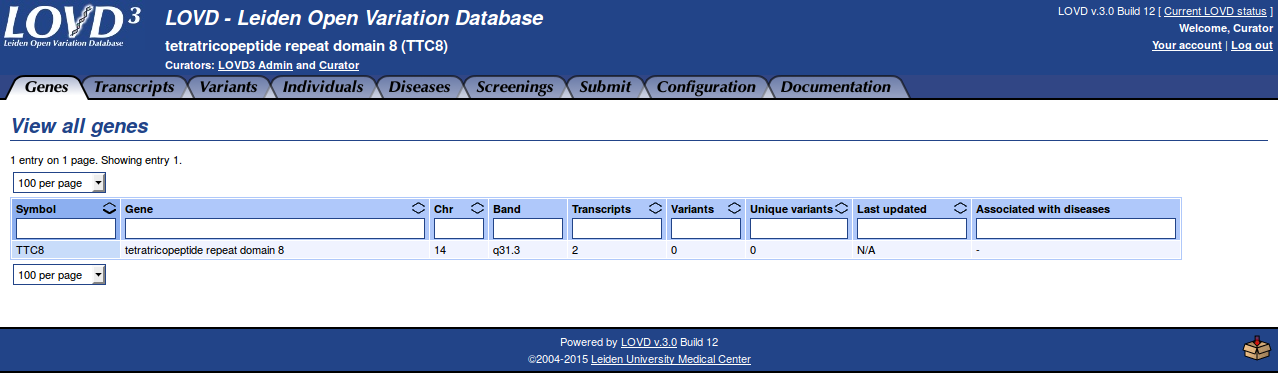
\includegraphics[width=\linewidth]
		   	 {/curate_gene/edit_gene_I.png}};
		  	\begin{scope}[x={(image.south east)},y={(image.north west)}]
		      \draw[red,ultra thick,rounded corners] (0.005,0.71) rectangle (0.075,0.8);
					\draw[<-, >=latex, \pointercolor, line width=\pointerwidth] (0.075,0.7505) to node[black]{A} (0.175,0.7505);
		      \draw[red,ultra thick,rounded corners] (0.12,0.845) rectangle (0.36,0.915);
					\draw[<-, >=latex, \pointercolor, line width=\pointerwidth] (0.36,0.88) to node[black]{B} (0.46,0.88);
		      \draw[red,ultra thick,rounded corners] (0.005,0.30) rectangle (0.32,0.37);
					\draw[<-, >=latex, \pointercolor, line width=\pointerwidth] (0.32,0.335) to node[black]{C} (0.42,0.335);
					%\drawgrid %help grid when positioning the boxes and pointers
		  	\end{scope}
			\end{tikzpicture}}
	  \caption{Via the Genes menu tab (A), you can go to the ``View gene'' page.
	  If in the header no gene is selected (B), then you are directed to ``View all genes''.\newline
	  Click on a gene (C) to go to the ``View gene'' page to see details of a gene. 
		If a gene is selected in the header and you click the Genes menu tab, 
		 you are directed to the ``View gene'' page, see figure \ref{fig:edit_gene_II}.}
		\label{fig:edit_gene_I}
  \end{shaded}
\end{figure}

\begin{figure}[ht]
  \begin{shaded}
		\frame{
			\begin{tikzpicture}
		  	\node[anchor=south west,inner sep=0] (image) at (0,0) {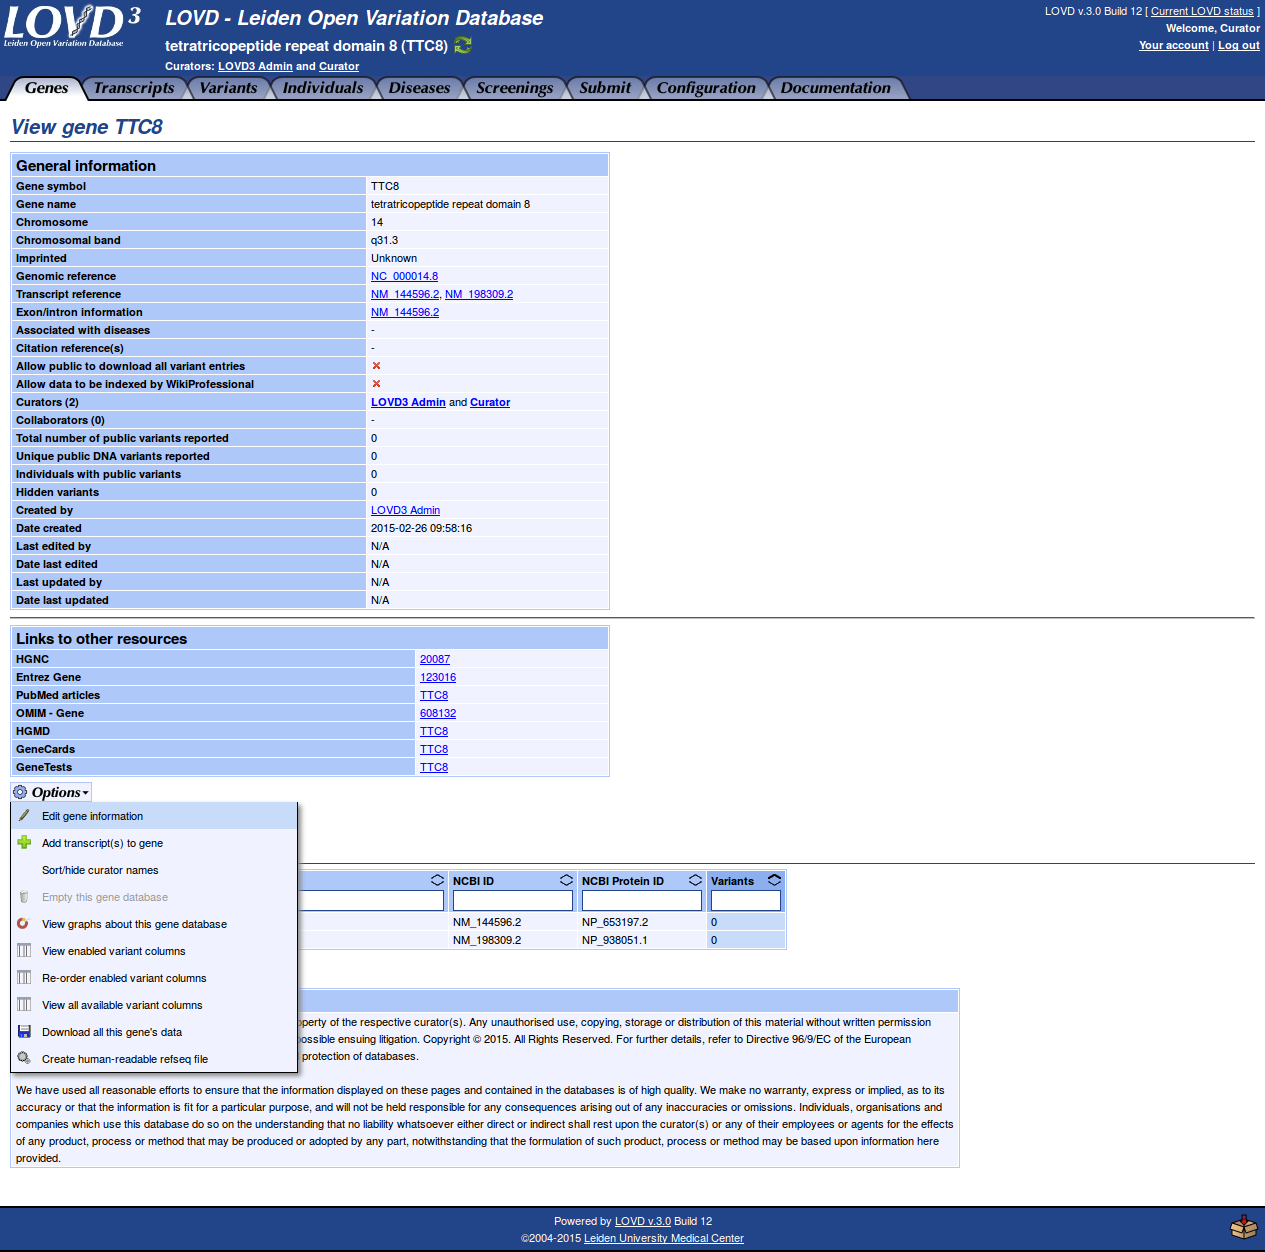
\includegraphics[width=\linewidth]
		   	 {/curate_gene/edit_gene_II.png}};
		  	\begin{scope}[x={(image.south east)},y={(image.north west)}]
		      \draw[red,ultra thick,rounded corners] (0.125,0.95) rectangle (0.38,0.975);
					\draw[<-, >=latex, \pointercolor, line width=\pointerwidth] (0.38,0.9615) to node[black]{A} (0.48,0.9615);
		      \draw[red,ultra thick,rounded corners] (0.005,0.915) rectangle (0.075,0.94);
					\draw[<-, >=latex, \pointercolor, line width=\pointerwidth] (0.075,0.9275) to node[black]{B} (0.175,0.9275);
		      \draw[red,ultra thick,rounded corners] (0.005,0.34) rectangle (0.17,0.36);
					\draw[<-, >=latex, \pointercolor, line width=\pointerwidth] (0.17,0.35) to node[black]{C} (0.27,0.35);
					%\drawgrid %help grid when positioning the boxes and pointers
		  	\end{scope}
			\end{tikzpicture}}
	  \caption{If a gene is selected in the header (A) and you click the Genes menu tab (B), 
	   you are directed to the ``View gene'' page.\newline
		On the ``View gene'' page, click the Options drop down menu and select ``Edit gene information'' (C).}
		\label{fig:edit_gene_II}
  \end{shaded}
\end{figure}

\begin{figure}[ht]
	\centering
  \begin{shaded}
		\frame{
			\begin{tikzpicture}
		  	\node[anchor=south west,inner sep=0] (image) at (0,0) {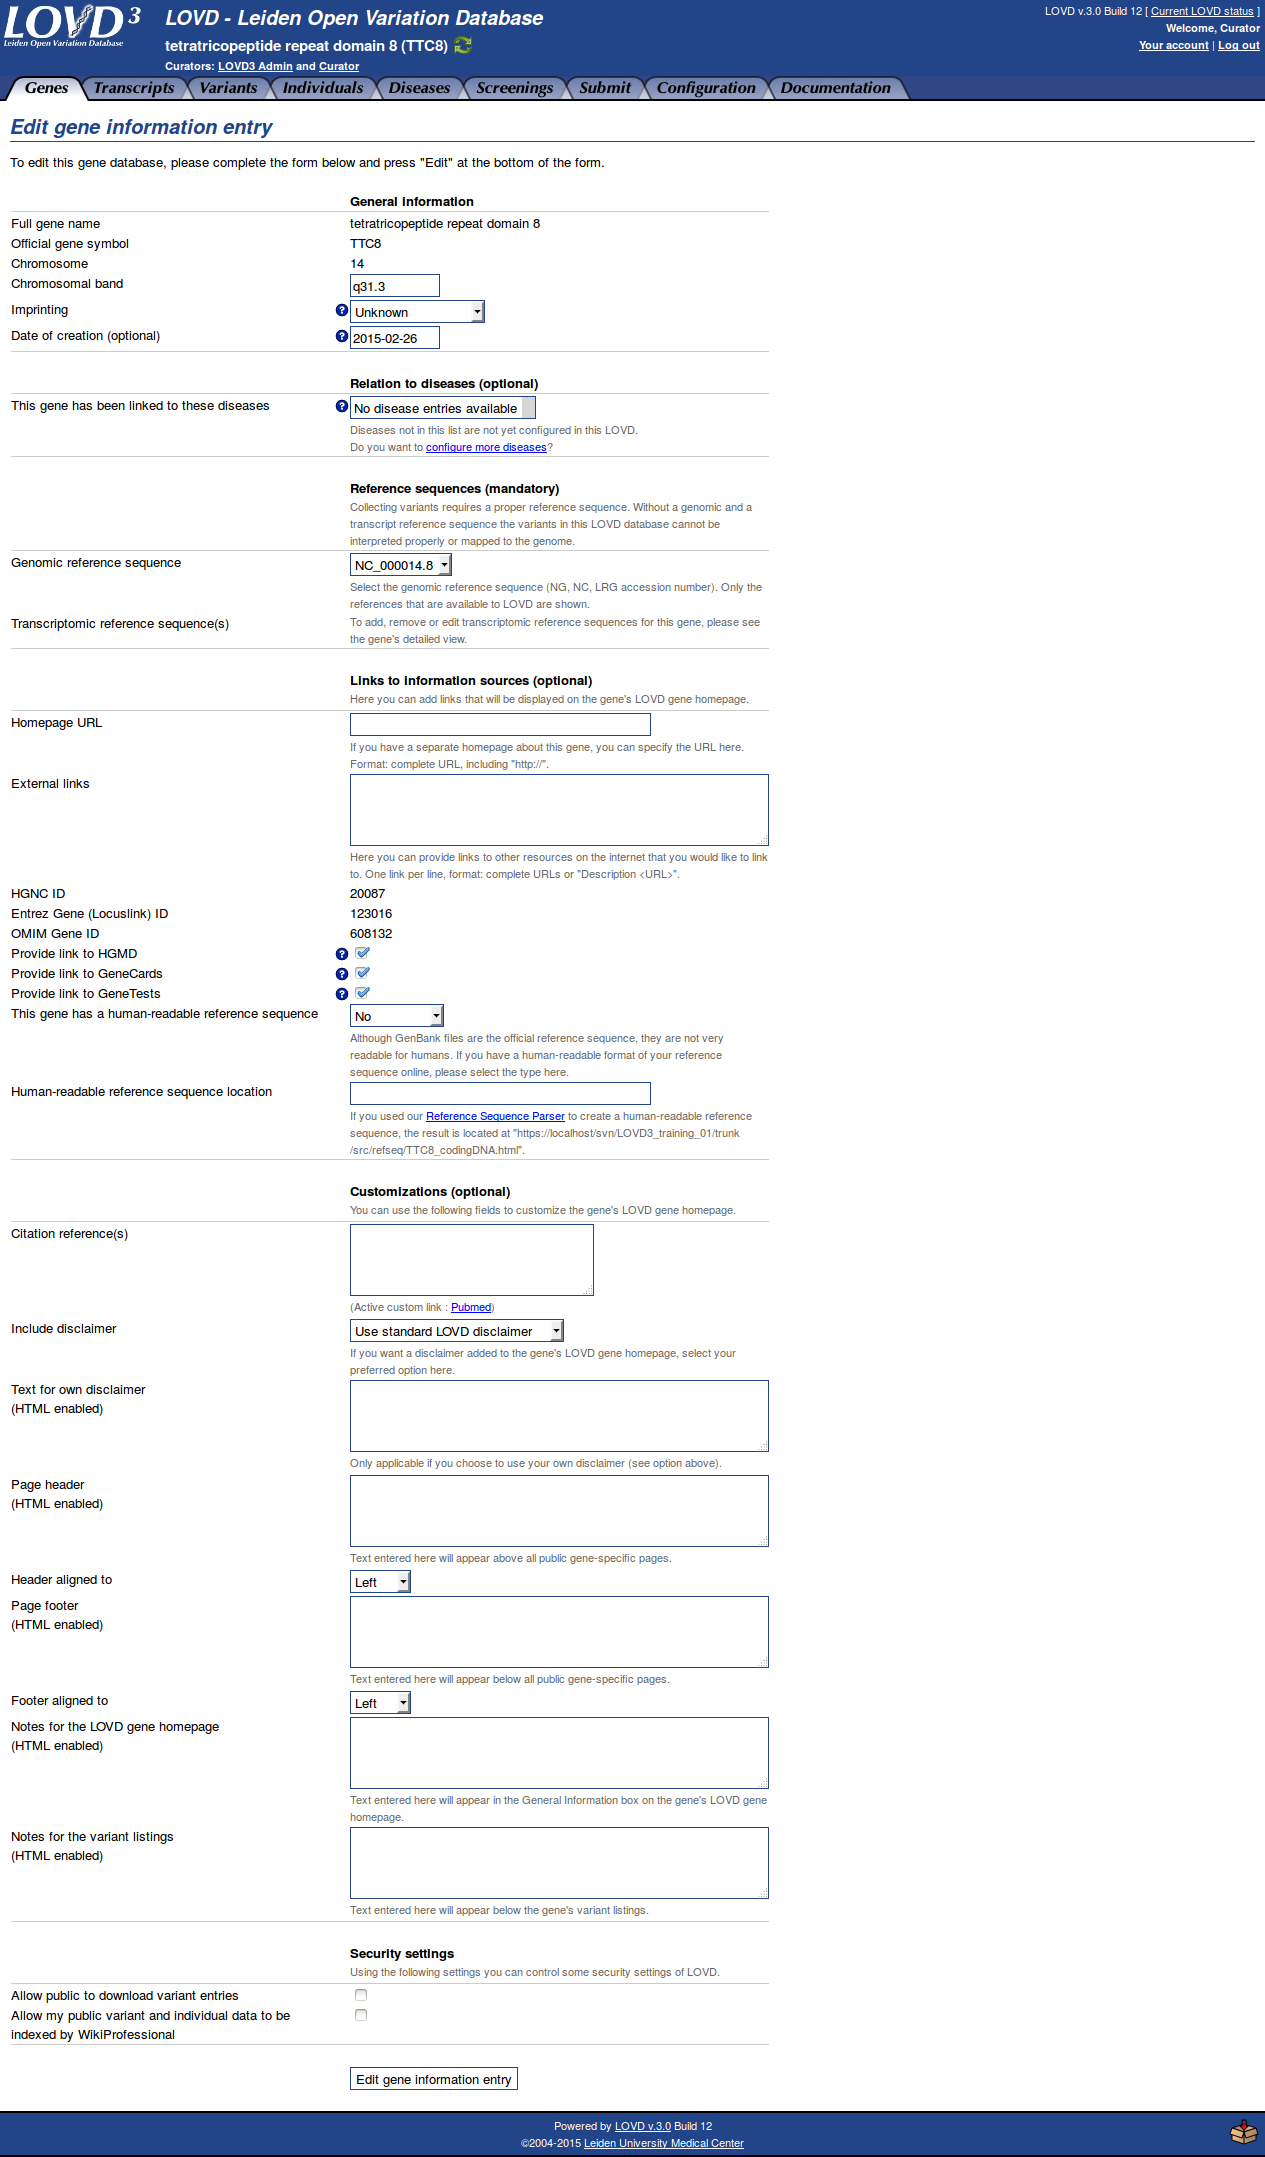
\includegraphics[height=0.85\textheight]
		   	 {/curate_gene/edit_gene_III.png}};
		  	\begin{scope}[x={(image.south east)},y={(image.north west)}]
		      \draw[red,ultra thick,rounded corners] (0.255,0.785) rectangle (0.45,0.83);
					\draw[<-, >=latex, \pointercolor, line width=\pointerwidth] (0.45,0.8075) to node[black]{A} (0.55,0.8075);
					%\drawgrid %help grid when positioning the boxes and pointers
		  	\end{scope}
			\end{tikzpicture}}
	  \caption{Look around and add or change things if you wish.
	  This gene does not have a relation to disease, yet. 
	  As an example we will add a related disease to this gene.\newline
	  There are two ways to add a disease and link this disease to a gene. 
	  The first method is demonstrated below; the second method is explained in chapter ``\nameref{chap:create_disease}''.
	  Click ``configure more diseases'' to create a new disease (A).}
		\label{fig:edit_gene_III}
  \end{shaded}
\end{figure}

\begin{figure}[ht]
  \begin{shaded}
		\frame{
			\begin{tikzpicture}
		  	\node[anchor=south west,inner sep=0] (image) at (0,0) {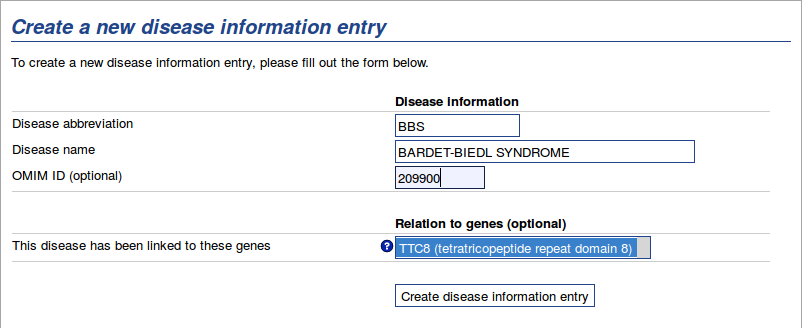
\includegraphics[width=\linewidth]
		   	 {/curate_gene/edit_gene_IV.png}};
		  	\begin{scope}[x={(image.south east)},y={(image.north west)}]
		      \draw[red,ultra thick,rounded corners] (0.47,0.40) rectangle (0.88,0.72);
					\draw[<-, >=latex, \pointercolor, line width=\pointerwidth] (0.47,0.56) to node[black]{A} (0.37,0.56);
		      \draw[red,ultra thick,rounded corners] (0.47,0.20) rectangle (0.82,0.36);
					\draw[<-, >=latex, \pointercolor, line width=\pointerwidth] (0.47,0.28) to node[black]{B} (0.37,0.28);
		      \draw[red,ultra thick,rounded corners] (0.47,0.05) rectangle (0.76,0.15);
					\draw[<-, >=latex, \pointercolor, line width=\pointerwidth] (0.47,0.1) to node[black]{C} (0.37,0.1);
					%\drawgrid %help grid when positioning the boxes and pointers
		  	\end{scope}
			\end{tikzpicture}}
	  \caption{To create a new disease, fill in the disease abbreviation, name and OMIM ID fields (A).\newline
		Note that the OMIM ID field is an unique field. 
		Therefore you can not use the same OMIM ID with different disease names.\newline
		To make a relation between this new disease select a gene, in our example TTC8 (B).
	  When you are curator of more genes, you can select a range of genes.\newline
		When you are ready, click ``Create disease information entry'' (C).}
		\label{fig:edit_gene_IV}
  \end{shaded}
\end{figure}

\begin{figure}[ht]
  \begin{shaded}
		\frame{
			\begin{tikzpicture}
		  	\node[anchor=south west,inner sep=0] (image) at (0,0) {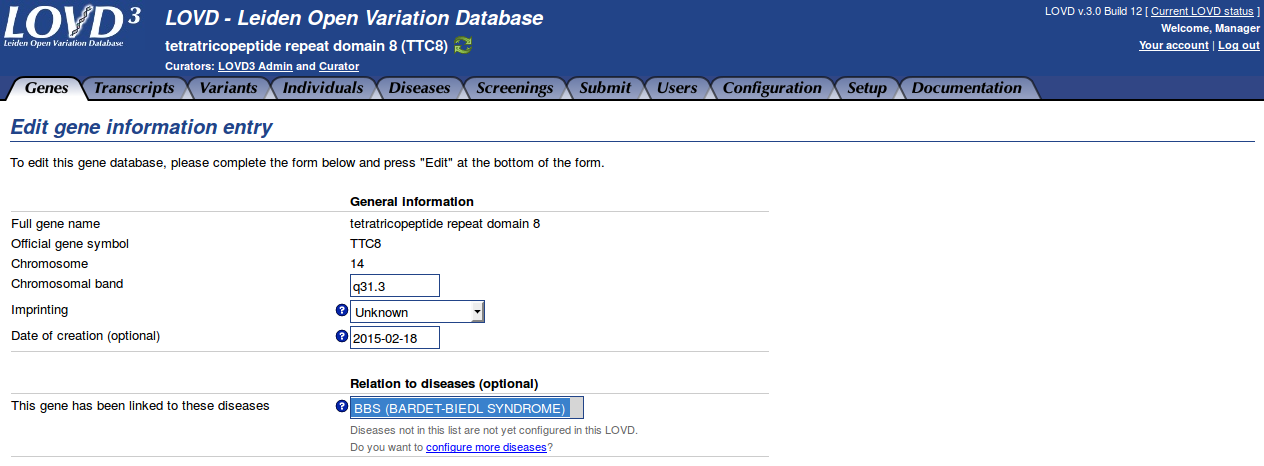
\includegraphics[width=\linewidth]
		   	 {/curate_gene/edit_gene_V.png}};
		  	\begin{scope}[x={(image.south east)},y={(image.north west)}]
		      \draw[red,ultra thick,rounded corners] (0.25,0.0) rectangle (0.51,0.20);
					\draw[<-, >=latex, \pointercolor, line width=\pointerwidth] (0.51,0.1) to node[black]{A} (0.61,0.1);
					%\drawgrid %help grid when positioning the boxes and pointers
		  	\end{scope}
			\end{tikzpicture}}
		\vskip 3 mm
		\frame{
			\begin{tikzpicture}
		  	\node[anchor=south west,inner sep=0] (image) at (0,0) {
\includegraphics[width=\linewidth]
		   	 {/curate_gene/edit_gene_VI.png}};
		  	\begin{scope}[x={(image.south east)},y={(image.north west)}]
		      \draw[red,ultra thick,rounded corners] (0.26,0.250) rectangle (0.43,0.45);
					\draw[<-, >=latex, \pointercolor, line width=\pointerwidth] (0.43,0.35) to node[black]{B} (0.53,0.35);
					%\drawgrid %help grid when positioning the boxes and pointers
		  	\end{scope}
			\end{tikzpicture}}
	  \caption{Gene TTC8 now has a relation to disease Bardet-Biedl Syndrome (A). \newline
	  Note that when you have more diseases in your installation, the diseases are ordered by abbreviation.
	  If a diseases entry has no abbreviation, it is listed below the disease with abbreviation. \newline
		When you have finished modifying the gene information, 
		 click ``Edit gene information entry'' to save the changes (B).}
		\label{fig:edit_gene_V}
  \end{shaded}
\end{figure}

\chapter{Creating a disease}
\label{chap:create_disease}
The objective of this chapter is:
\begin{enumerate}
	\item 
	Create disease information and add a disease to a gene via the Disease menu tab.
\end{enumerate}

\begin{figure}[ht]
  \begin{shaded}
		\frame{
			\begin{tikzpicture}
		  	\node[anchor=south west,inner sep=0] (image) at (0,0) {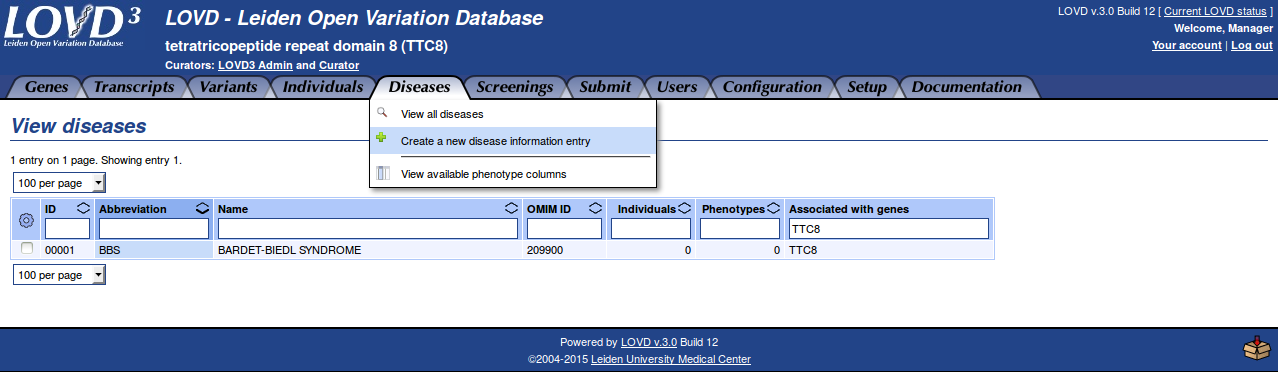
\includegraphics[width=\linewidth]
		   	 {/curate_gene/create_disease_I.png}};
		  	\begin{scope}[x={(image.south east)},y={(image.north west)}]
		      \draw[red,ultra thick,rounded corners] (0.285,0.58) rectangle (0.48,0.66);
					\draw[<-, >=latex, \pointercolor, line width=\pointerwidth] (0.48,0.62) to node[black]{} (0.58,0.62);
					%\drawgrid %help grid when positioning the boxes and pointers
		  	\end{scope}
			\end{tikzpicture}}
	  \caption{Create a disease via ``Create a new disease information entry'' on the Diseases menu tab drop 
	   down menu.}
		\label{fig:create_disease_I}
  \end{shaded}
\end{figure}

\begin{figure}[ht]
  \begin{shaded}
		\frame{
			\begin{tikzpicture}
		  	\node[anchor=south west,inner sep=0] (image) at (0,0) {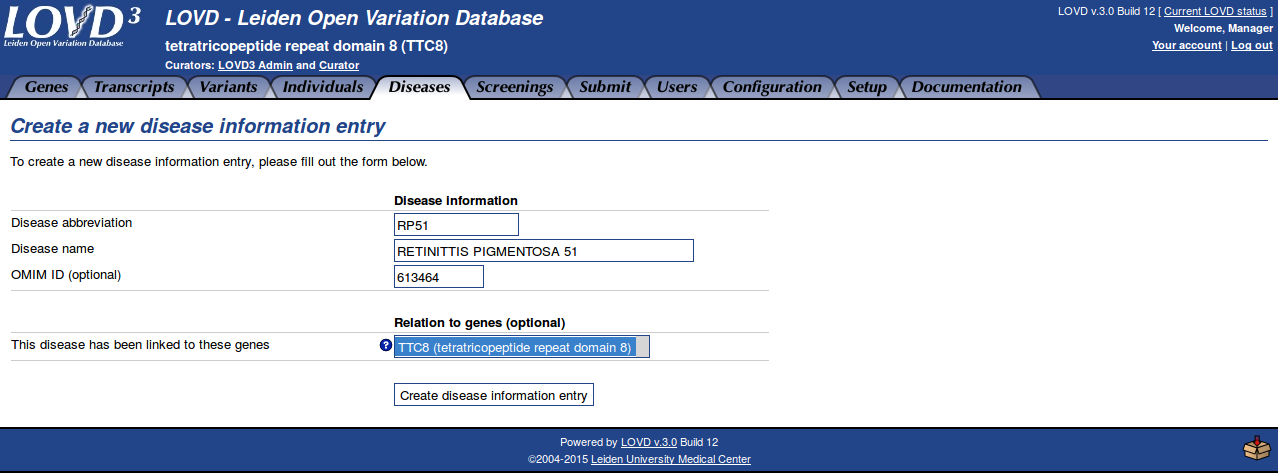
\includegraphics[width=\linewidth]
		   	 {/curate_gene/create_disease_II.png}};
		  	\begin{scope}[x={(image.south east)},y={(image.north west)}]
		      \draw[red,ultra thick,rounded corners] (0.29,0.37) rectangle (0.55,0.60);
					\draw[<-, >=latex, \pointercolor, line width=\pointerwidth] (0.55,0.485) to node[black]{A} (0.65,0.485);
		      \draw[red,ultra thick,rounded corners] (0.29,0.23) rectangle (0.52,0.34);
					\draw[<-, >=latex, \pointercolor, line width=\pointerwidth] (0.52,0.285) to node[black]{B} (0.62,0.285);
		      \draw[red,ultra thick,rounded corners] (0.29,0.14) rectangle (0.48,0.19);
					\draw[<-, >=latex, \pointercolor, line width=\pointerwidth] (0.48,0.165) to node[black]{C} (0.58,0.165);
					%\drawgrid %help grid when positioning the boxes and pointers
		  	\end{scope}
			\end{tikzpicture}}
	  \caption{To create a disease, fill in the disease abbreviation, name and OMIM ID fields (A).\newline
		To make a relation to this new disease, select a gene, in our example TTC8 (B).
		When you are curator of more genes, you can select a range of genes.\newline
		When you are ready, click ``Create disease information entry''(C).}
		\label{fig:create_disease_II}
  \end{shaded}
\end{figure}

\begin{figure}[ht]
  \begin{shaded}
		\frame{
			\begin{tikzpicture}
		  	\node[anchor=south west,inner sep=0] (image) at (0,0) {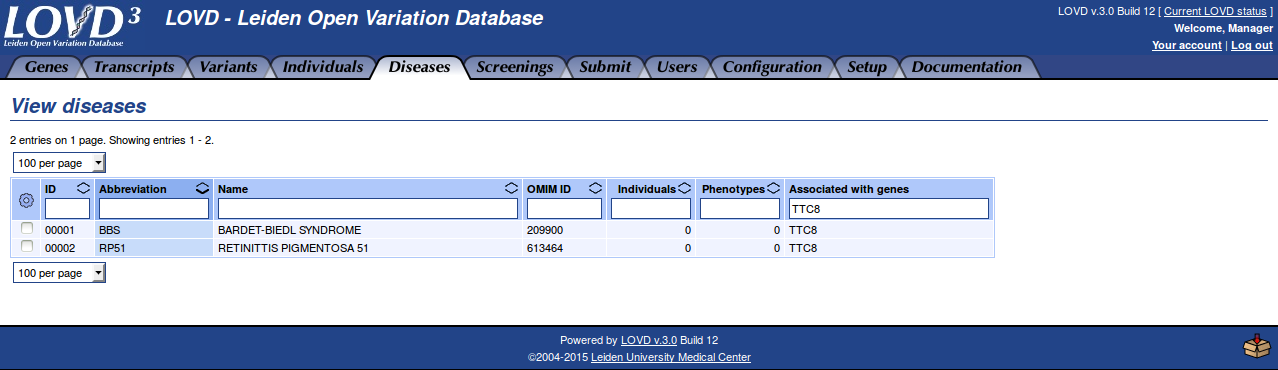
\includegraphics[width=\linewidth]
		   	 {/curate_gene/create_disease_III.png}};
		  	\begin{scope}[x={(image.south east)},y={(image.north west)}]
		      \draw[red,ultra thick,rounded corners] (0.285,0.77) rectangle (0.37,0.855);
					\draw[<-, >=latex, \pointercolor, line width=\pointerwidth] (0.37,0.8125) to node[black]{A} (0.47,0.8125);
		      \draw[red,ultra thick,rounded corners] (0.615,0.30) rectangle (0.75,0.515);
					\draw[<-, >=latex, \pointercolor, line width=\pointerwidth] (0.75,0.4075) to node[black]{B} (0.85,0.4075);
					%\drawgrid %help grid when positioning the boxes and pointers
		  	\end{scope}
			\end{tikzpicture}}
	  \caption{We now have created two diseases, one in chapter ``\nameref{chap:edit_gene_database}'' and one in 
	   this chapter.
	  To see them click the Diseases menu tab (A).
	  You can see both diseases are associated with the TTC8 gene(B).}
		\label{fig:create_disease_III}
  \end{shaded}
\end{figure}










\chapter{Reference sequences and the reference sequence parser}
The objective of this chapter is:
\begin{enumerate}
	\item 
	Create an HTML page of the DNA reference sequence with exon/intron boundaries, up- and downstream and 
	 intronic sequences.
\end{enumerate}
To start this chapter:
\begin{itemize}
	\item 
	Log in as Curator (with for every one the same username: curator, password: curator1).
\end{itemize}

\begin{figure}[ht]
  \begin{shaded}
		\frame{
			\begin{tikzpicture}
		  	\node[anchor=south west,inner sep=0] (image) at (0,0) {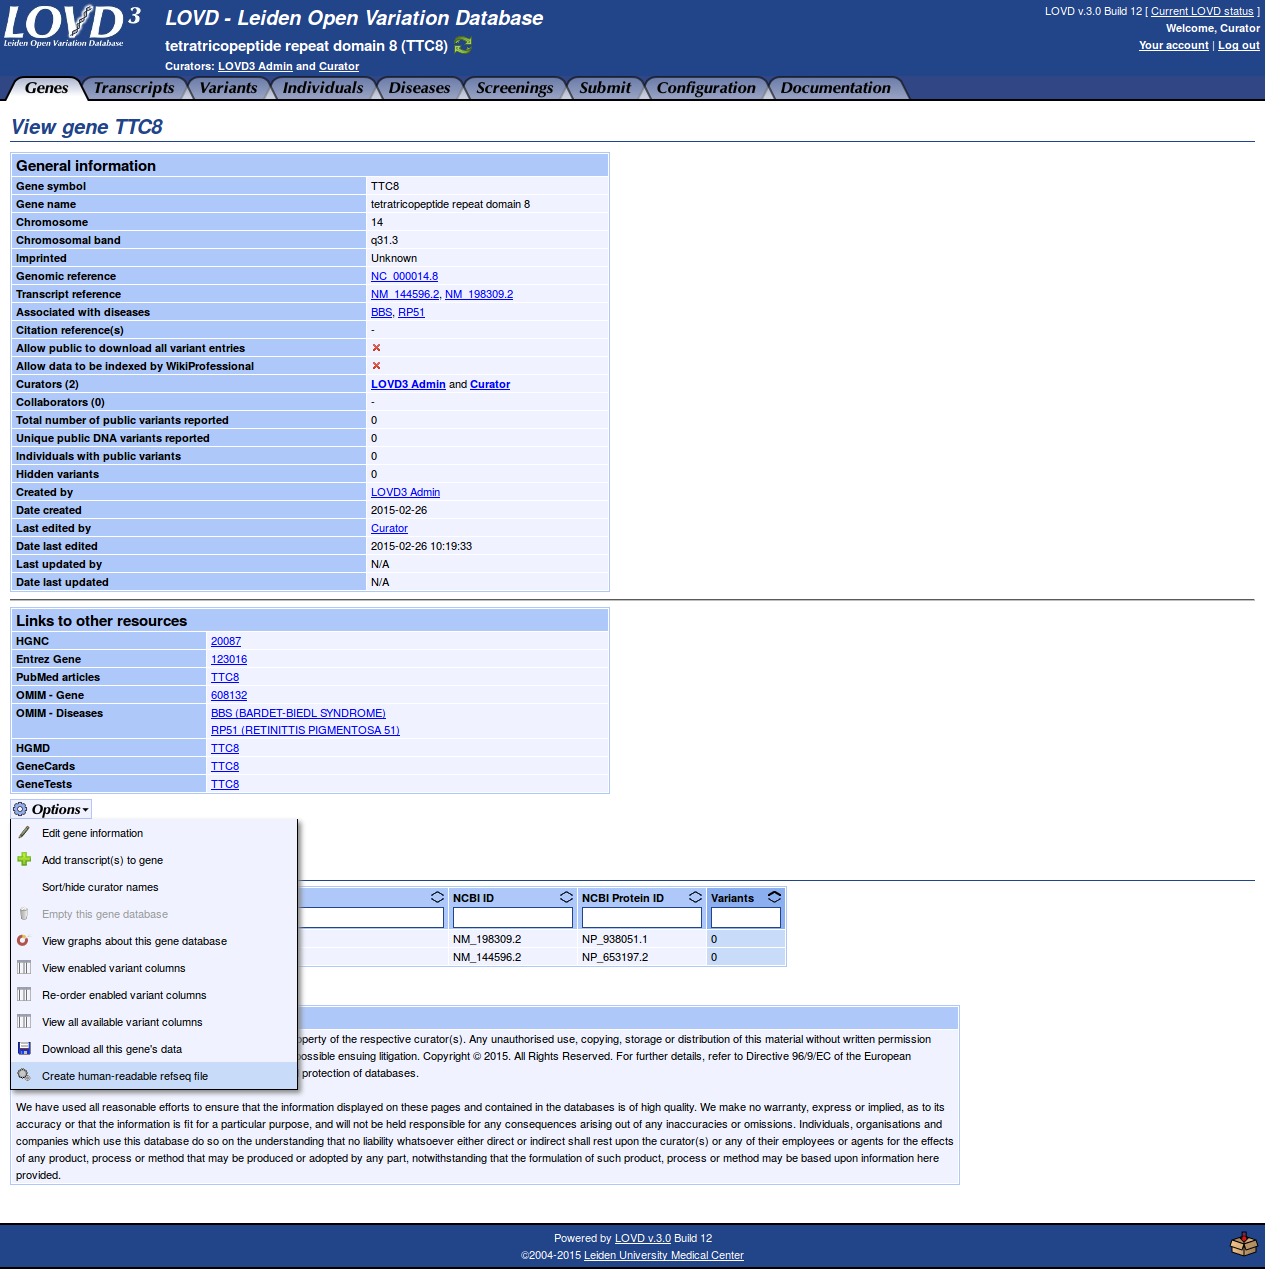
\includegraphics[width=\linewidth]
		   	 {/curate_gene/create_refseq_page_I.png}};
		  	\begin{scope}[x={(image.south east)},y={(image.north west)}]
		      \draw[red,ultra thick,rounded corners] (0.005,0.915) rectangle (0.07,0.945);
					\draw[<-, >=latex, \pointercolor, line width=\pointerwidth] (0.07,0.93) to node[black]{A} (0.17,0.93);
		      \draw[red,ultra thick,rounded corners] (0.005,0.14) rectangle (0.235,0.17);
					\draw[<-, >=latex, \pointercolor, line width=\pointerwidth] (0.235,0.155) to node[black]{B} (0.335,0.155);
					%\drawgrid %help grid when positioning the boxes and pointers
		  	\end{scope}
			\end{tikzpicture}}
	  \caption{Go to the Genes menu tab (A).
	 	If in the header no gene is selected, you are directed to ``View all genes''.  
	 	You have to select a gene first, see figure \ref{fig:edit_gene_I}.
	  On the ``View gene'' page, click the Options drop down menu and select ``Create human-readable refseq file'' (B).
		A popup screen will appear.}
		\label{fig:create_refseq_page_I}
  \end{shaded}
\end{figure}

\begin{figure}[ht]
  \begin{shaded}
		\frame{
			\begin{tikzpicture}
		  	\node[anchor=south west,inner sep=0] (image) at (0,0) {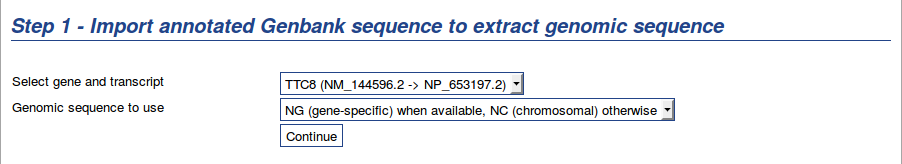
\includegraphics[width=\linewidth]
		   	 {/curate_gene/create_refseq_page_II.png}};
		  	\begin{scope}[x={(image.south east)},y={(image.north west)}]
					%\drawgrid %help grid when positioning the boxes and pointers
		  	\end{scope}
			\end{tikzpicture}}
	  \caption{Select gene and transcript and which sequence you want to use. 
	  In our example choose ``TTC8(NM\_144596.2 -> NP\_653197.2)'' and ``NG (gene-specific) when available, 
	   NC (chromosomal) otherwise''.
   	Continue when ready.}
		\label{fig:create_refseq_page_II}
  \end{shaded}
\end{figure}

\begin{figure}[ht]
  \begin{shaded}
		\frame{
			\begin{tikzpicture}
		  	\node[anchor=south west,inner sep=0] (image) at (0,0) {
\includegraphics[width=\linewidth]
		   	 {/curate_gene/create_refseq_page_III.png}};
		  	\begin{scope}[x={(image.south east)},y={(image.north west)}]
					%\drawgrid %help grid when positioning the boxes and pointers
		  	\end{scope}
			\end{tikzpicture}}
	  \caption{Continue to next step.}
		\label{fig:create_refseq_page_III}
  \end{shaded}
\end{figure}

\begin{figure}[ht]
  \begin{shaded}
		\frame{
			\begin{tikzpicture}
		  	\node[anchor=south west,inner sep=0] (image) at (0,0) {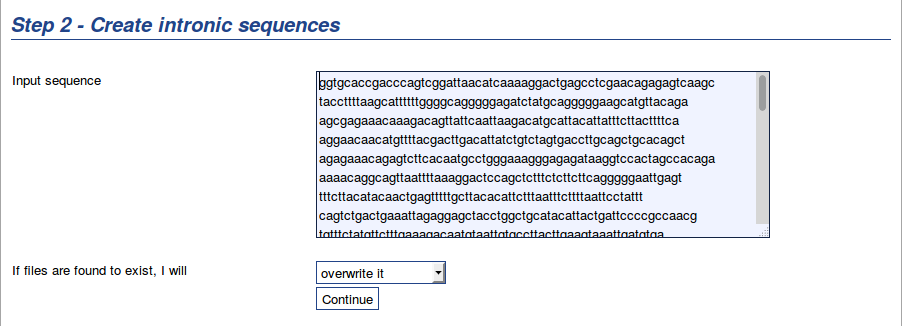
\includegraphics[width=\linewidth]
		   	 {/curate_gene/create_refseq_page_IV.png}};
		  	\begin{scope}[x={(image.south east)},y={(image.north west)}]
					%\drawgrid %help grid when positioning the boxes and pointers
		  	\end{scope}
			\end{tikzpicture}}
	  \caption{Choose between ``overwrite'', ``rename the old file'' or ``skip the file''. 
	  In our example choose overwrite it.
	  Since it is the first time we create intronic sequences, there are no old files to overwrite.}
		\label{fig:create_refseq_page_IV}
  \end{shaded}
\end{figure}

\begin{figure}[ht]
  \begin{shaded}
		\frame{
			\begin{tikzpicture}
		  	\node[anchor=south west,inner sep=0] (image) at (0,0) {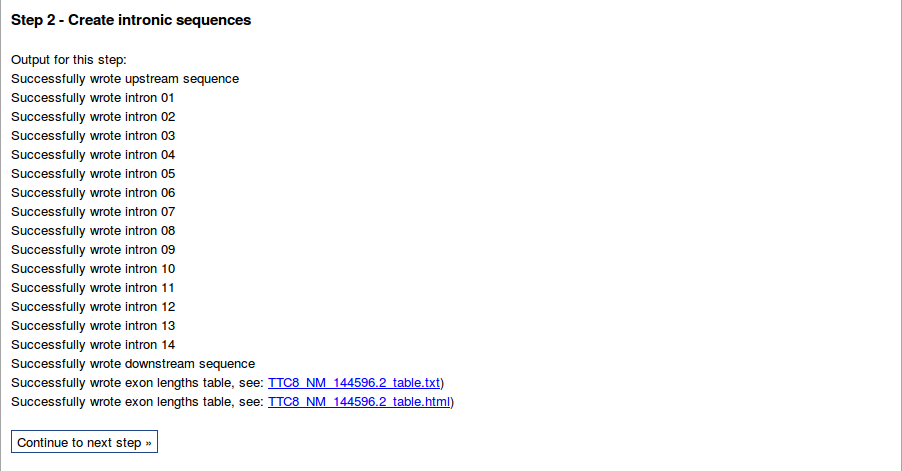
\includegraphics[width=\linewidth]
		   	 {/curate_gene/create_refseq_page_V.png}};
		  	\begin{scope}[x={(image.south east)},y={(image.north west)}]
					\draw[<-, >=latex, \pointercolor, line width=\pointerwidth] (0.45,0.2) to node[black]{A} (0.45,0.4);
					\draw[<-, >=latex, \pointercolor, line width=\pointerwidth] (0.51,0.14) to node[black]{B} (0.61,0.14);
	 		  		\node[anchor=south west,inner sep=0] (image) at (0.35,0.45) {\fbox{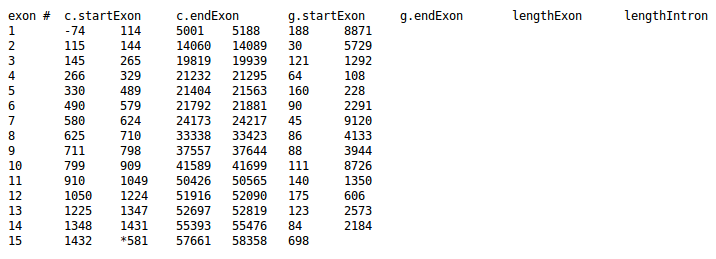
\includegraphics[width=0.6\linewidth]
			   	 {/curate_gene/create_refseq_page_VI.png}}};
	 		  	\node[anchor=south west,inner sep=0] (image) at (0.61,0) {\fbox{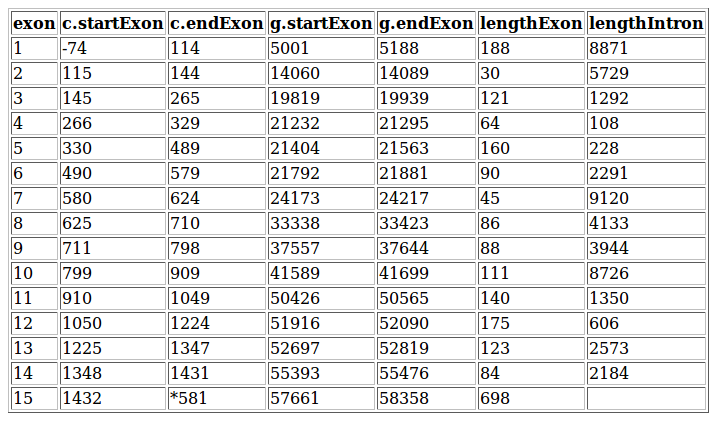
\includegraphics[width=0.37\linewidth]
			   	 {/curate_gene/create_refseq_page_VII.png}}};
					%\drawgrid %help grid when positioning the boxes and pointers
		  	\end{scope}
			\end{tikzpicture}}
	  \caption{The exon lengths table is created. 
	  You can click the link to see the exon lengths in text format (A) or in HTML format (B).}
		\label{fig:create_refseq_page_V}
  \end{shaded}
\end{figure}

\begin{figure}[ht]
  \begin{shaded}
		\frame{
			\begin{tikzpicture}
		  	\node[anchor=south west,inner sep=0] (image) at (0,0) {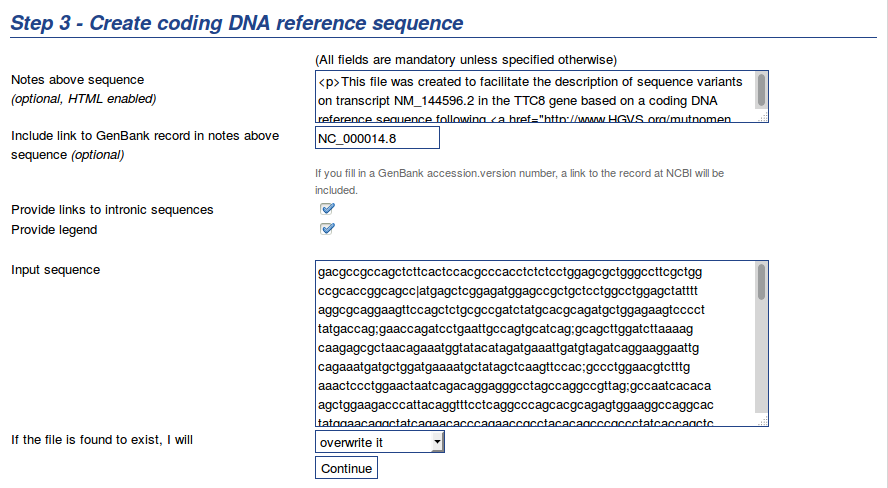
\includegraphics[width=\linewidth]
		   	 {/curate_gene/create_refseq_page_VIII.png}};
		  	\begin{scope}[x={(image.south east)},y={(image.north west)}]
					%\drawgrid %help grid when positioning the boxes and pointers
		  	\end{scope}
			\end{tikzpicture}}
	  \caption{Choose between ``overwrite'', ``rename the old file'' or ``skip the file''. 
	  In our example choose overwrite it.
	  Since it is the first time we create intronic sequences, there are no old files to overwrite.}
		\label{fig:create_refseq_page_VIII}
  \end{shaded}
\end{figure}

\begin{figure}[ht]
  \begin{shaded}
		\frame{
			\begin{tikzpicture}
		  	\node[anchor=south west,inner sep=0] (image) at (0,0) {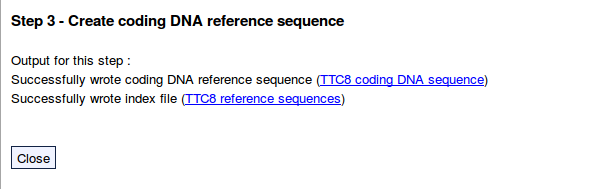
\includegraphics[width=\linewidth]
		   	 {/curate_gene/create_refseq_page_IX.png}};
		  	\begin{scope}[x={(image.south east)},y={(image.north west)}]
					\draw[<-, >=latex, \pointercolor, line width=\pointerwidth] (0.83,0.57) to node[black]{A} (0.93,0.57);
					\draw[<-, >=latex, \pointercolor, line width=\pointerwidth] (0.6,0.475) to node[black]{B} (0.7,0.475);
					%\drawgrid %help grid when positioning the boxes and pointers
		  	\end{scope}
			\end{tikzpicture}}
	  \caption{The coding DNA sequence (A, see figure \ref{fig:create_refseq_page_X}) is created.
	  The second link (B) shows all transcripts for which the reference sequence parser has been run.
	  If there is just one, it redirects you to the coding sequence.}
		\label{fig:create_refseq_page_IX}
  \end{shaded}
\end{figure}

\begin{figure}[ht]
	\centering
  \begin{shaded}
		\frame{
			\begin{tikzpicture}
		  	\node[anchor=south west,inner sep=0] (image) at (0,0) {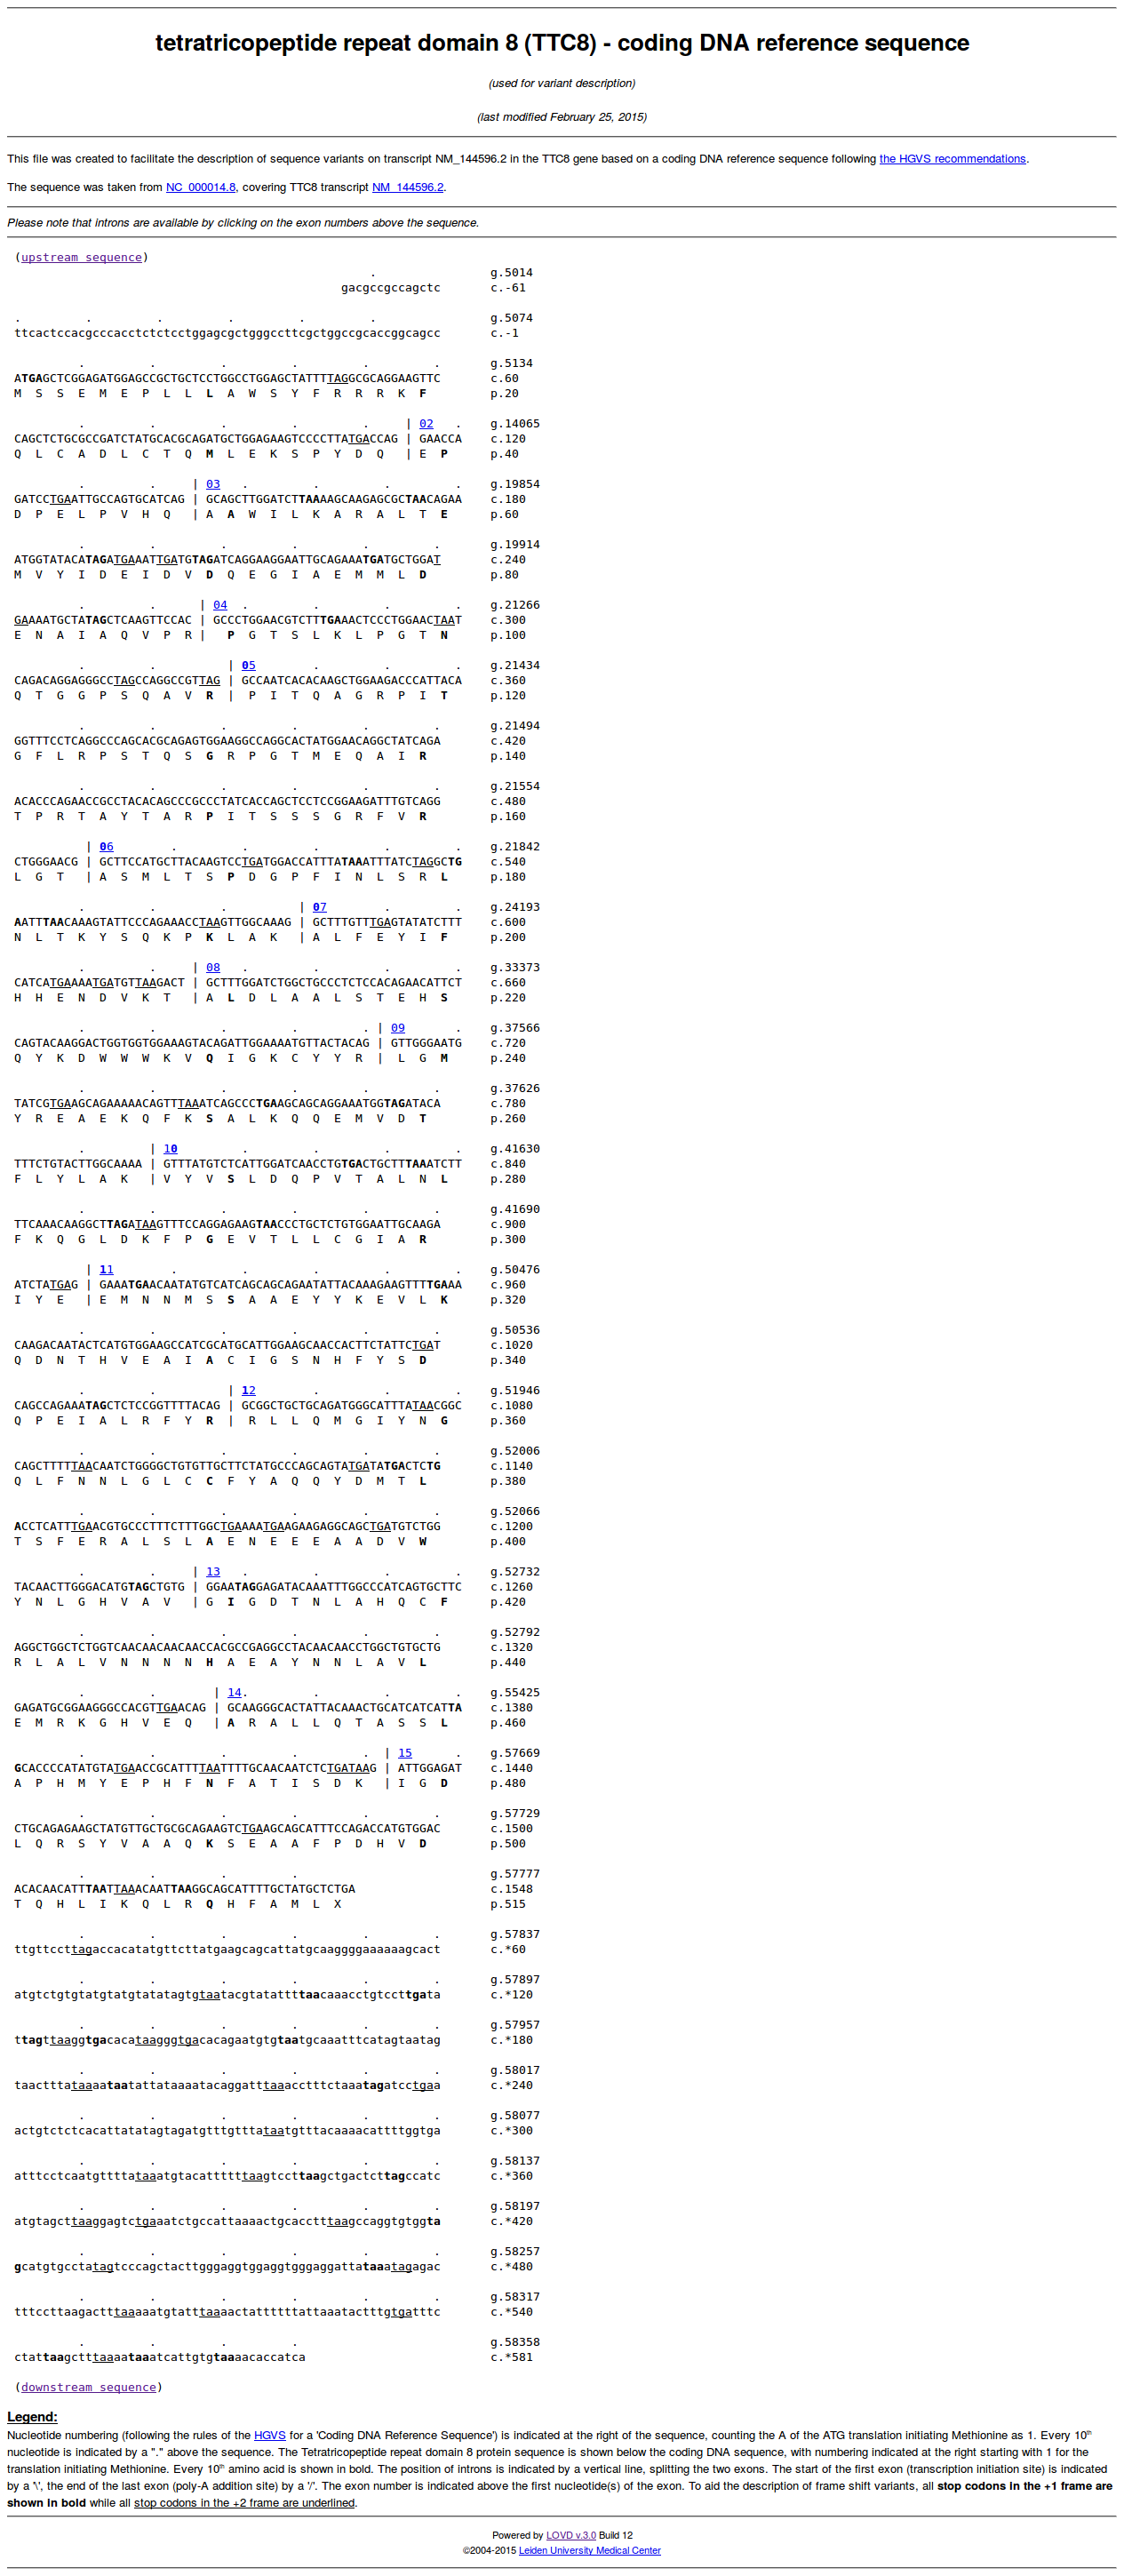
\includegraphics[height=0.93\textheight]
		   	 {/curate_gene/create_refseq_page_X.png}};
		  	\begin{scope}[x={(image.south east)},y={(image.north west)}]
					%\drawgrid %help grid when positioning the boxes and pointers
		  	\end{scope}
			\end{tikzpicture}}
	  \caption{The TTC8 (NM\_144596.2) coding DNA reference sequence.}
		\label{fig:create_refseq_page_X}
  \end{shaded}
\end{figure}










\chapter{Editing columns and legends}
\label{edit_columns_legends}
The objectives of this chapter are:
\begin{enumerate}
	\item 
	Enable a new Variant on Transcript custom data column
	\item 
	Edit the legend of the new column
	\item
	Change column order
\end{enumerate}
To start this chapter:
\begin{itemize}
	\item
	Please check existing description for existing custom columns and do not deviate too much. 
	In general, non-standard use of custom columns raises a lot of confusion.
	\item
	Log in as Curator (username: curator, password: curator1).
\end{itemize}

\begin{figure}[ht]
  \begin{shaded}
		\frame{
			\begin{tikzpicture}
		  	\node[anchor=south west,inner sep=0] (image) at (0,0) {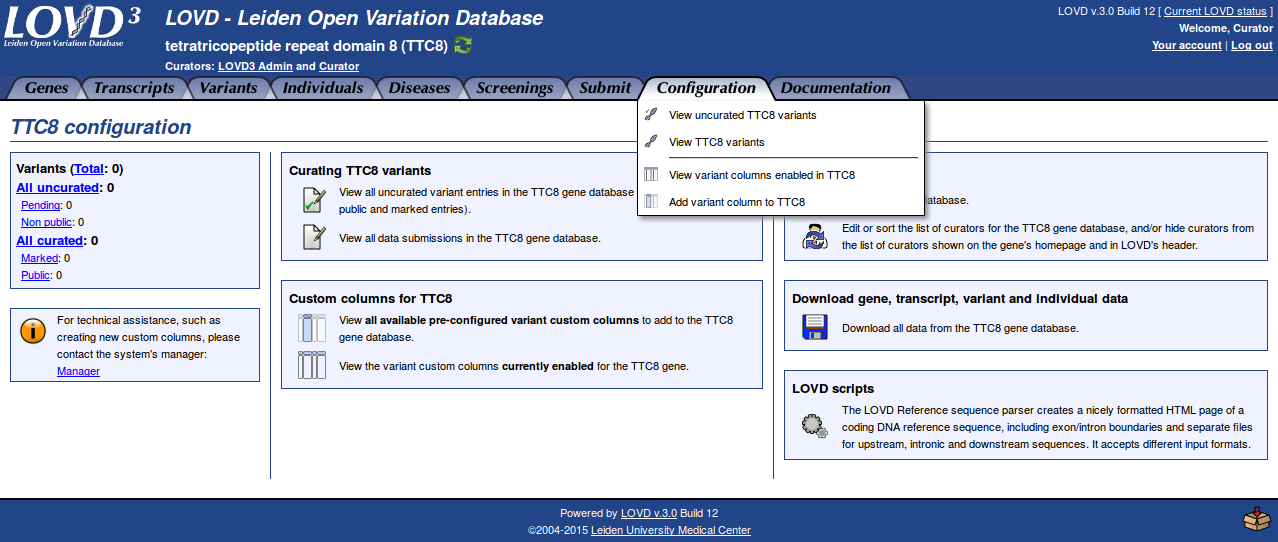
\includegraphics[width=\linewidth]
		   	 {/curate_gene/edit_column_I.png}};
		  	\begin{scope}[x={(image.south east)},y={(image.north west)}]
		      \draw[red,ultra thick,rounded corners] (0.495,0.595) rectangle (0.65,0.655);
					\draw[<-, >=latex, \pointercolor, line width=\pointerwidth] (0.65,0.625) to node[black]{A} (0.75,0.625);
		      \draw[red,ultra thick,rounded corners] (0.22,0.36) rectangle (0.6,0.47);
					\draw[<-, >=latex, \pointercolor, line width=\pointerwidth] (0.6,0.425) to node[black]{B} (0.7,0.425);
					%\drawgrid %help grid when positioning the boxes and pointers
		  	\end{scope}
			\end{tikzpicture}}
	  \caption{On the ``Browse VariantOnTranscript custom data columns'' page you can see an overview of available 
	   custom columns.
	   You can go there directly via ``Add variant column to TTC8'' on the Configuration menu tab (A). 
		Or from the configuration area, click the ``View all available pre-configured variant custom columns\ldots'' 
		 link listed under	``Custom columns for TTC8''(B).}
		\label{fig:edit_column_I}
  \end{shaded}
\end{figure}


\begin{figure}[ht]
  \begin{shaded}
		\frame{
			\begin{tikzpicture}
		  	\node[anchor=south west,inner sep=0] (image) at (0,0) {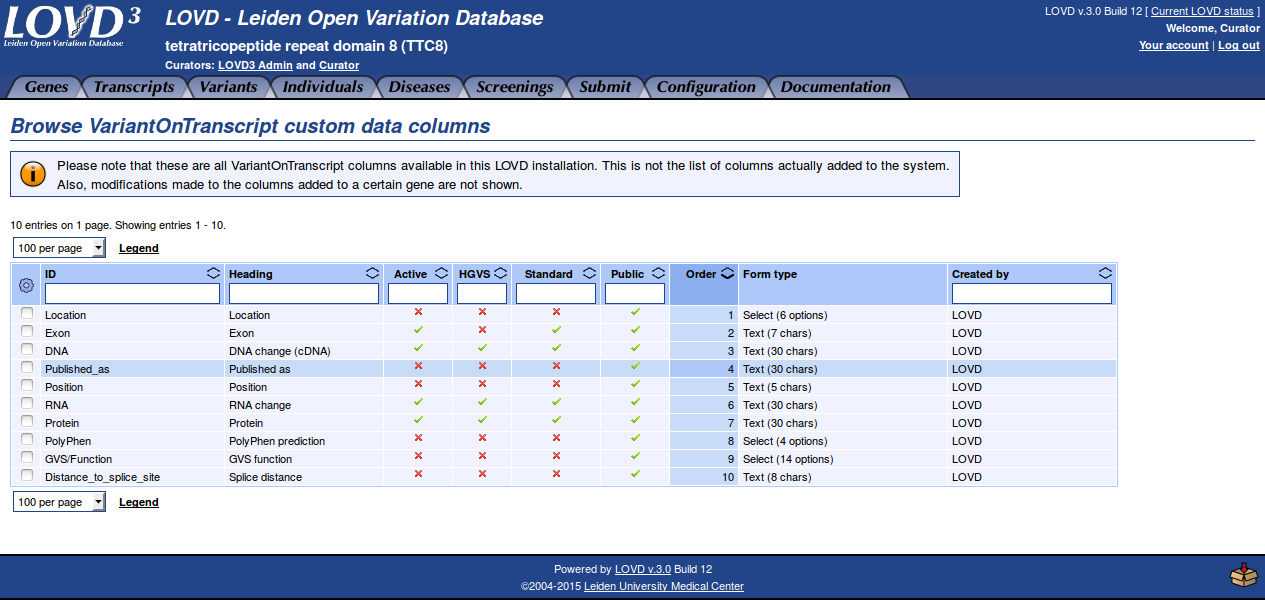
\includegraphics[width=\linewidth]
		   	 {/curate_gene/edit_column_II.png}};
		  	\begin{scope}[x={(image.south east)},y={(image.north west)}]
		      \draw[red,ultra thick,rounded corners] (0.02,0.37) rectangle (0.35,0.405);
					\draw[<-, >=latex, \pointercolor, line width=\pointerwidth] (0.35,0.3875) to node[black]{} (0.45,0.3875);
					%\drawgrid %help grid when positioning the boxes and pointers
		  	\end{scope}
			\end{tikzpicture}}
	  \caption{You can see that the custom column ``Published\_as'' is not (yet) active.
	  We are going to enable this custom column.
	  Click on ``Published\_as''.}
		\label{fig:edit_column_II}
  \end{shaded}
\end{figure}

\begin{figure}[ht]
  \begin{shaded}
		\frame{
			\begin{tikzpicture}
		  	\node[anchor=south west,inner sep=0] (image) at (0,0) {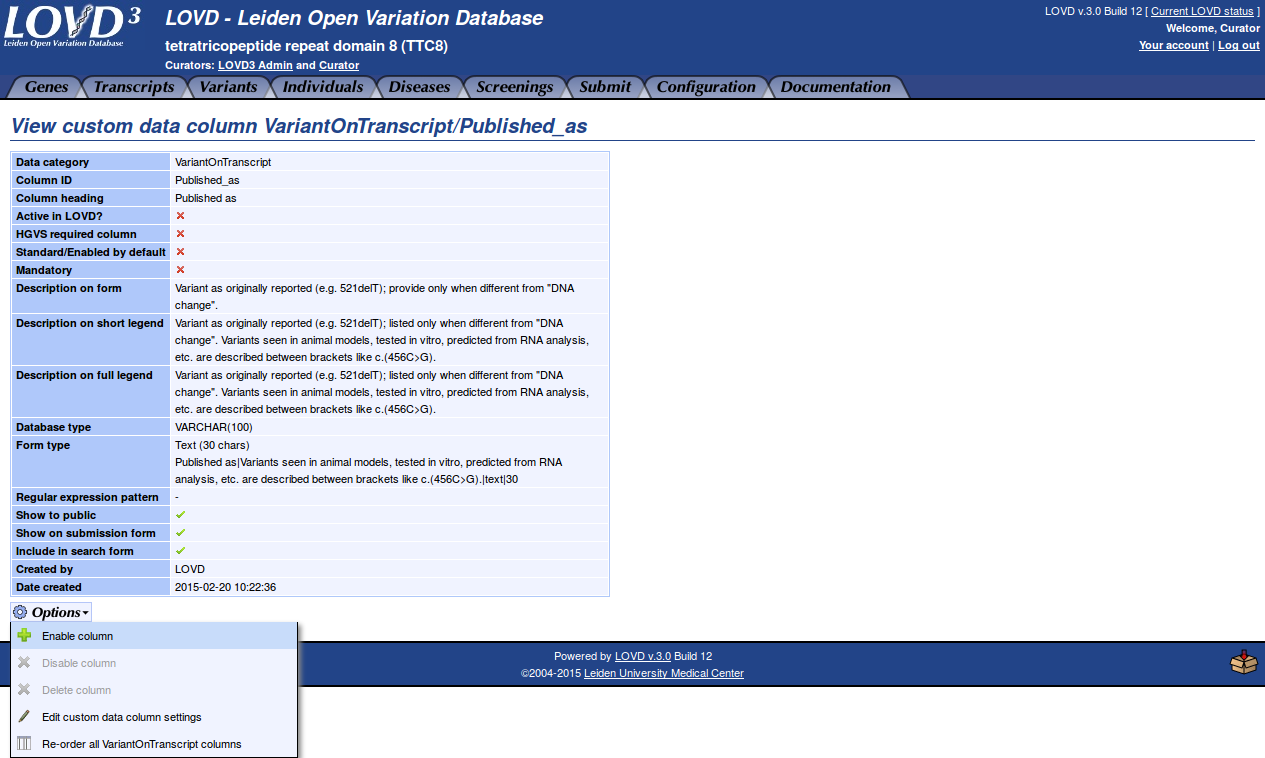
\includegraphics[width=\linewidth]
		   	 {/curate_gene/edit_column_III.png}};
		  	\begin{scope}[x={(image.south east)},y={(image.north west)}]
		      \draw[red,ultra thick,rounded corners] (0.005,0.145) rectangle (0.235,0.18);
					\draw[<-, >=latex, \pointercolor, line width=\pointerwidth] (0.235,0.1625) to node[black]{} (0.335,0.1625);
					%\drawgrid %help grid when positioning the boxes and pointers
		  	\end{scope}
			\end{tikzpicture}}
	  \caption{Click the Options drop down menu and select ``Enable column''.}
		\label{fig:edit_column_III}
  \end{shaded}
\end{figure}

\begin{figure}[ht]
  \begin{shaded}
		\frame{
			\begin{tikzpicture}
		  	\node[anchor=south west,inner sep=0] (image) at (0,0) {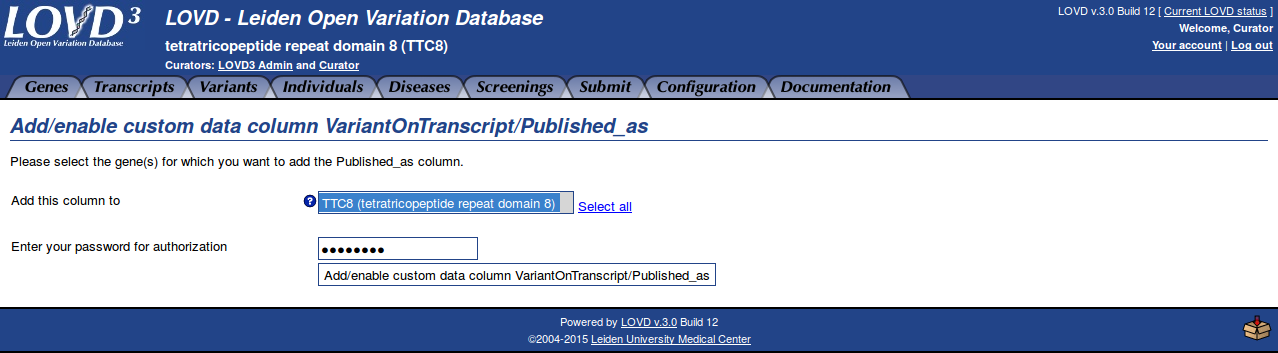
\includegraphics[width=\linewidth]
		   	 {/curate_gene/edit_column_IV.png}};
		  	\begin{scope}[x={(image.south east)},y={(image.north west)}]
		      %\drawgrid %help grid when positioning the boxes and pointers
		  	\end{scope}
			\end{tikzpicture}}
	  \caption{Select the gene to which you want to add this custom column. 
	  In this case we have only TTC8. 
	  When you are curator of more genes, you can select a range of genes.\newline
	  Confirm with your password and click ``Add/enable custom data column VariantOnTranscript/Published\_as''.}
		\label{fig:edit_column_IV}
  \end{shaded}
\end{figure}

\begin{figure}[ht]
  \begin{shaded}
		\frame{
			\begin{tikzpicture}
		  	\node[anchor=south west,inner sep=0] (image) at (0,0) {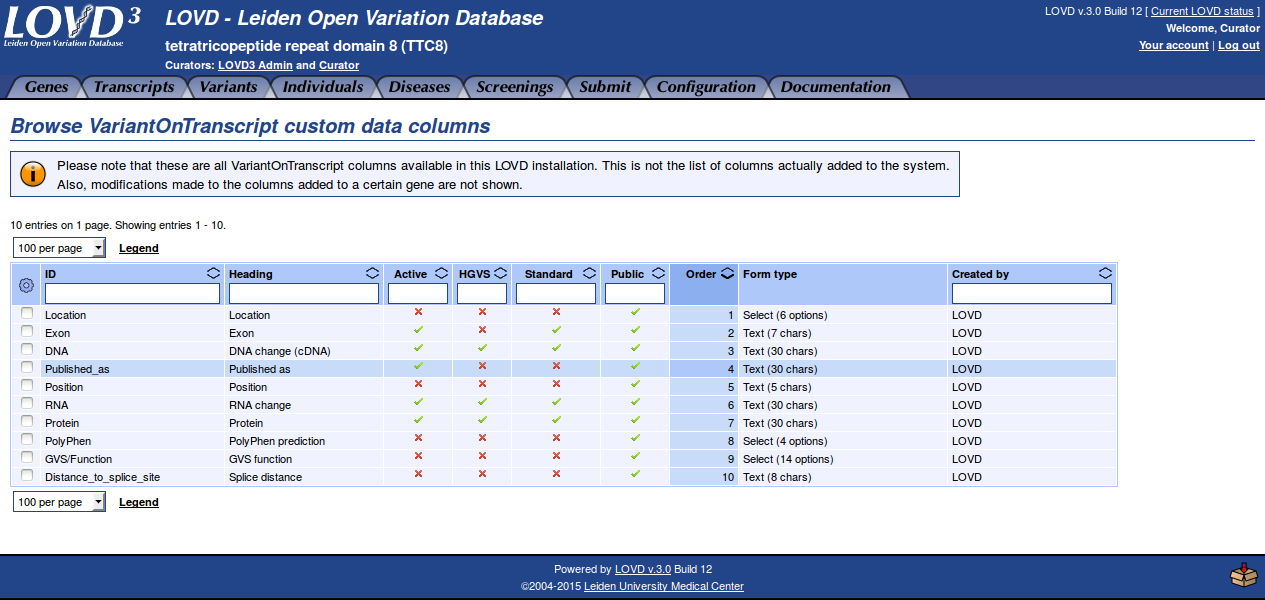
\includegraphics[width=\linewidth]
		   	 {/curate_gene/edit_column_V.png}};
		  	\begin{scope}[x={(image.south east)},y={(image.north west)}]
		      \draw[red,ultra thick,rounded corners] (0.02,0.365) rectangle (0.35,0.405);
					\draw[<-, >=latex, \pointercolor, line width=\pointerwidth] (0.35,0.385) to node[black]{} (0.45,0.385);
					%\drawgrid %help grid when positioning the boxes and pointers
		  	\end{scope}
			\end{tikzpicture}}
	  \caption{In the view ``Browse VariantOnTranscript custom data columns'' you can see that the published\_as custom
	   column has become active. }
		\label{fig:edit_column_V}
  \end{shaded}
\end{figure}

\begin{figure}[ht]
  \begin{shaded}
		\frame{
			\begin{tikzpicture}
		  	\node[anchor=south west,inner sep=0] (image) at (0,0) {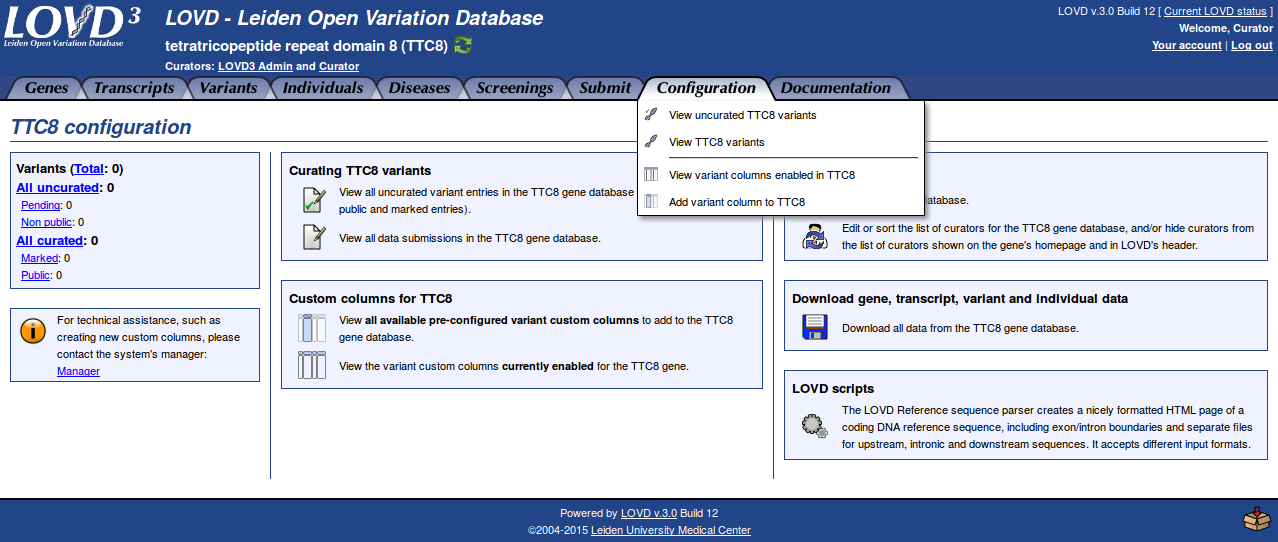
\includegraphics[width=\linewidth]
		   	 {/curate_gene/edit_column_I.png}};
		  	\begin{scope}[x={(image.south east)},y={(image.north west)}]
		      \draw[red,ultra thick,rounded corners] (0.495,0.655) rectangle (0.65,0.705);
					\draw[<-, >=latex, \pointercolor, line width=\pointerwidth] (0.65,0.68) to node[black]{A} (0.75,0.68);
		      \draw[red,ultra thick,rounded corners] (0.22,0.28) rectangle (0.6,0.36);
					\draw[<-, >=latex, \pointercolor, line width=\pointerwidth] (0.6,0.32) to node[black]{B} (0.7,0.32);
					%\drawgrid %help grid when positioning the boxes and pointers
		  	\end{scope}
			\end{tikzpicture}}
	  \caption{To change the custom column descriptions go to ``View variant columns enabled in TTC8''
	   via the Configuration menu tab (A). 
		Or from the configuration area, click the ``View the variant custom columns currently enabled for the TTC8 gene.'' 
		link listed under	``Custom columns for TTC8''(B).}
		\label{fig:edit_column_VI}
  \end{shaded}
\end{figure}

\begin{figure}[ht]
  \begin{shaded}
		\frame{
			\begin{tikzpicture}
		  	\node[anchor=south west,inner sep=0] (image) at (0,0) {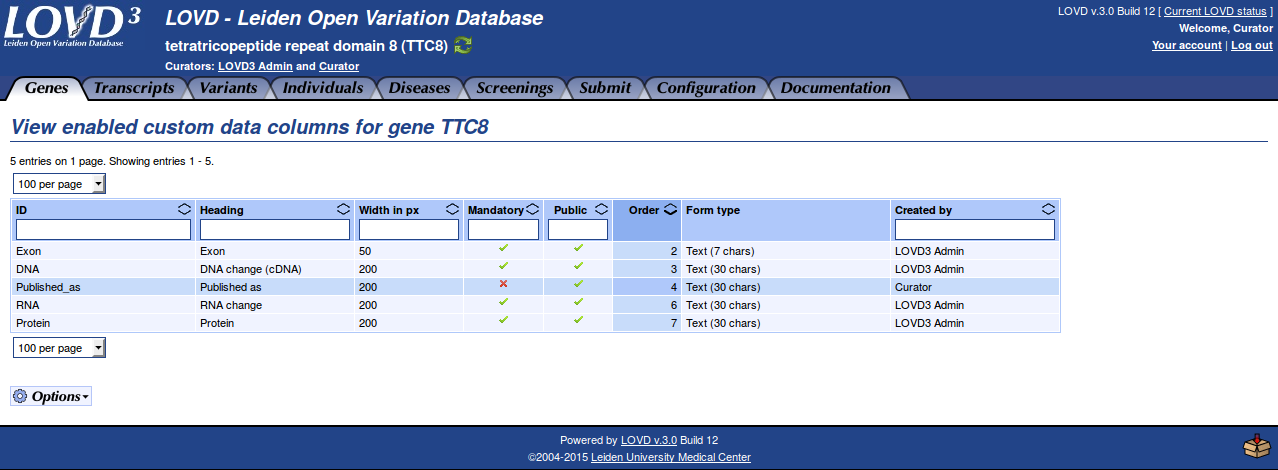
\includegraphics[width=\linewidth]
		   	 {/curate_gene/edit_column_VII.png}};
		  	\begin{scope}[x={(image.south east)},y={(image.north west)}]
		      \draw[red,ultra thick,rounded corners] (0.005,0.365) rectangle (0.25,0.41);
					\draw[<-, >=latex, \pointercolor, line width=\pointerwidth] (0.25,0.3875) to node[black]{} (0.35,0.3875);
					%\drawgrid %help grid when positioning the boxes and pointers
		  	\end{scope}
			\end{tikzpicture}}
	  \caption{On the ``View enabled custom data columns for the gene'' you can see an overview of the active custom 
	   data columns.
	  Click on custom column ``Published\_as''.}
		\label{fig:edit_column_VII}
  \end{shaded}
\end{figure}

\begin{figure}[ht]
  \begin{shaded}
		\frame{
			\begin{tikzpicture}
		  	\node[anchor=south west,inner sep=0] (image) at (0,0) {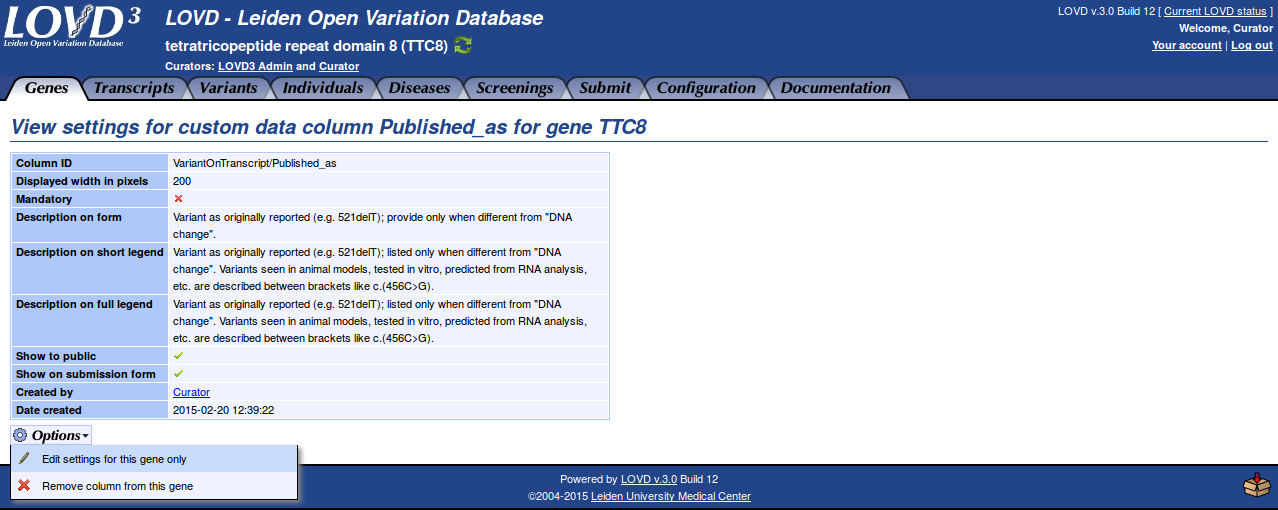
\includegraphics[width=\linewidth]
		   	 {/curate_gene/edit_column_VIII.png}};
		  	\begin{scope}[x={(image.south east)},y={(image.north west)}]
		      \draw[red,ultra thick,rounded corners] (0.005,0.08) rectangle (0.235,0.135);
					\draw[<-, >=latex, \pointercolor, line width=\pointerwidth] (0.235,0.1075) to node[black]{} (0.335,0.1075);
					%\drawgrid %help grid when positioning the boxes and pointers
		  	\end{scope}
			\end{tikzpicture}}
	  \caption{Click the Options drop down menu and select ``Edit settings for this gene only''.}
		\label{fig:edit_column_VIII}
  \end{shaded}
\end{figure}

\begin{figure}[ht]
  \begin{shaded}
		\frame{
			\begin{tikzpicture}
		  	\node[anchor=south west,inner sep=0] (image) at (0,0) {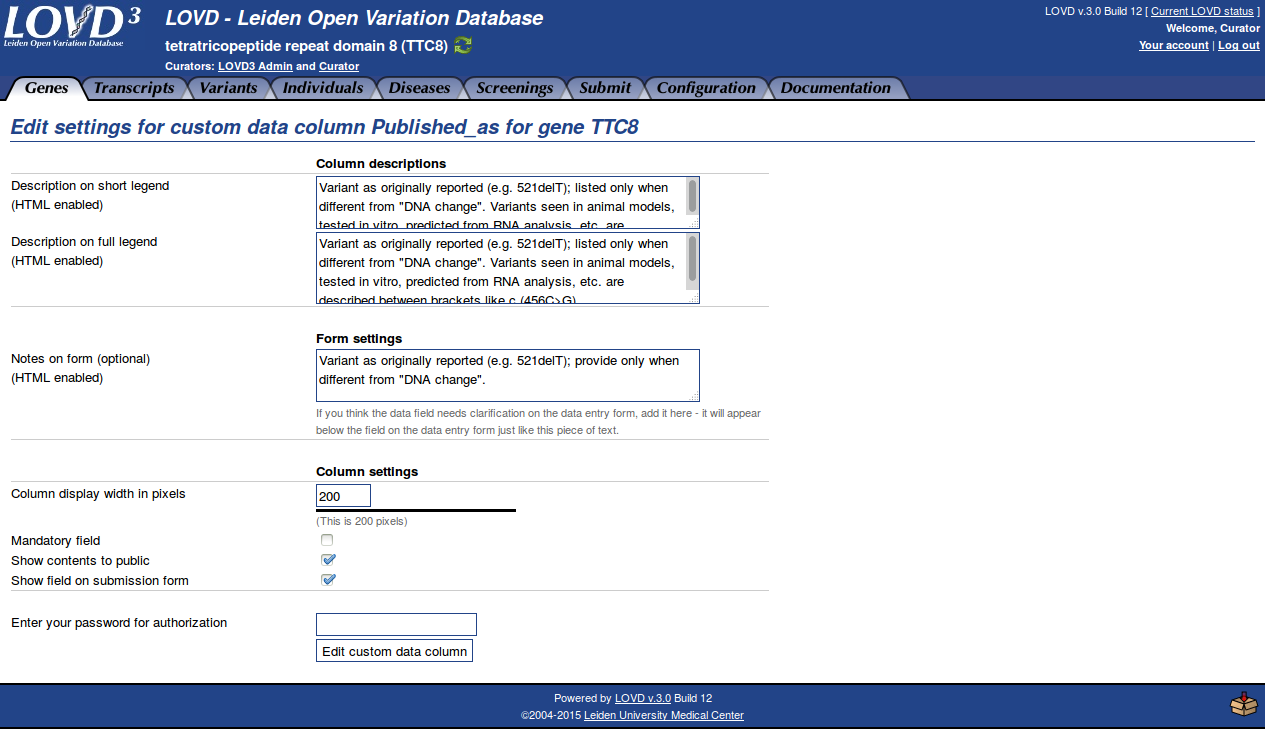
\includegraphics[width=\linewidth]
		   	 {/curate_gene/edit_column_IX.png}};
		  	\begin{scope}[x={(image.south east)},y={(image.north west)}]
		      \draw[red,ultra thick,rounded corners] (0.24,0.58) rectangle (0.56,0.79);
					\draw[<-, >=latex, \pointercolor, line width=\pointerwidth] (0.56,0.685) to node[black]{A} (0.66,0.685);
		      \draw[red,ultra thick,rounded corners] (0.24,0.09) rectangle (0.38,0.18);
					\draw[<-, >=latex, \pointercolor, line width=\pointerwidth] (0.38,0.135) to node[black]{B} (0.48,0.135);
					%\drawgrid %help grid when positioning the boxes and pointers
		  	\end{scope}
			\end{tikzpicture}}
	  \caption{Here you can change the ``Description on short legend'' and the ``Description on full legend''. 
	  Provide more information when available (A).\newline
	  When done, confirm with your password and click ``Edit custom data column'' (B). 
	  The results of these changes you can see in figure \ref{fig:submission_X}.}
		\label{fig:edit_column_IX}
  \end{shaded}
\end{figure}

\begin{figure}[ht]
  \begin{shaded}
		\frame{
			\begin{tikzpicture}
		  	\node[anchor=south west,inner sep=0] (image) at (0,0) {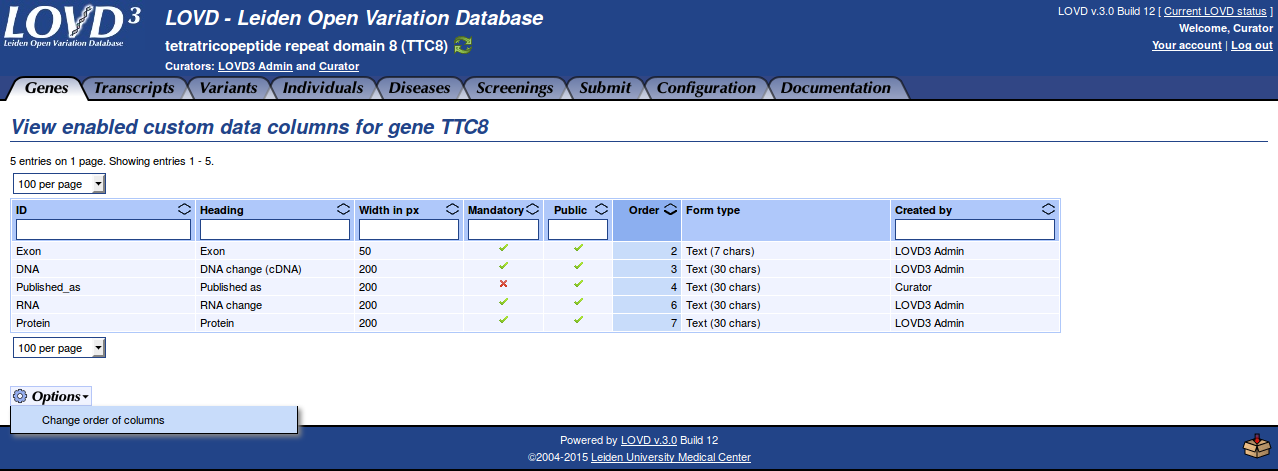
\includegraphics[width=\linewidth]
		   	 {/curate_gene/edit_column_X.png}};
		  	\begin{scope}[x={(image.south east)},y={(image.north west)}]
		      \draw[red,ultra thick,rounded corners] (0.005,0.08) rectangle (0.235,0.14);
					\draw[<-, >=latex, \pointercolor, line width=\pointerwidth] (0.235,0.11) to node[black]{} (0.335,0.11);
					%\drawgrid %help grid when positioning the boxes and pointers
		  	\end{scope}
			\end{tikzpicture}}
	  \caption{To change the order of custom data columns, go to ``View enabled custom data columns for gene TTC8'', 
	   see figure \ref{fig:edit_column_VI} how to get there.\newline
	  Click the Options drop down menu and select ``Change order of columns''.}
		\label{fig:edit_column_X}
  \end{shaded}
\end{figure}

\begin{figure}[ht]
  \begin{shaded}
		\frame{
			\begin{tikzpicture}
		  	\node[anchor=south west,inner sep=0] (image) at (0,0) {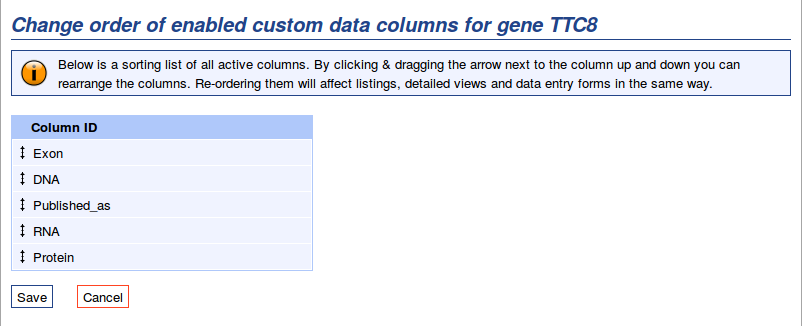
\includegraphics[width=\linewidth]
		   	 {/curate_gene/edit_column_XI.png}};
		  	\begin{scope}[x={(image.south east)},y={(image.north west)}]
		      %\draw[red,ultra thick,rounded corners] (0.015,0.16) rectangle (0.04,0.57);
					%\draw[<-, >=latex, \pointercolor, line width=\pointerwidth] (0.04,0.5) to node[black]{} (0.14,0.5);
					%\drawgrid %help grid when positioning the boxes and pointers
		  	\end{scope}
			\end{tikzpicture}}
	  \caption{You can click and drag the arrows in front of the column ID and move the columns up and down.
	  Click save when ready.
	  The results of these changes you can see in figure \ref{fig:submission_X}.}
		\label{fig:edit_column_XI}
  \end{shaded}
\end{figure}










\chapter{Submission}
The objectives of this chapter are:
\begin{enumerate}
	\item 
	Update a submitters registration
	\item 
	Submit an individual, phenotype, screening and variant.
\end{enumerate}
To start this chapter:
\begin{itemize}
	\item
	Log in as Submitter (username: submitter, password: submitter1).
\end{itemize}

\begin{figure}[ht]
  \begin{shaded}
		\frame{
			\begin{tikzpicture}
		  	\node[anchor=south west,inner sep=0] (image) at (0,0) {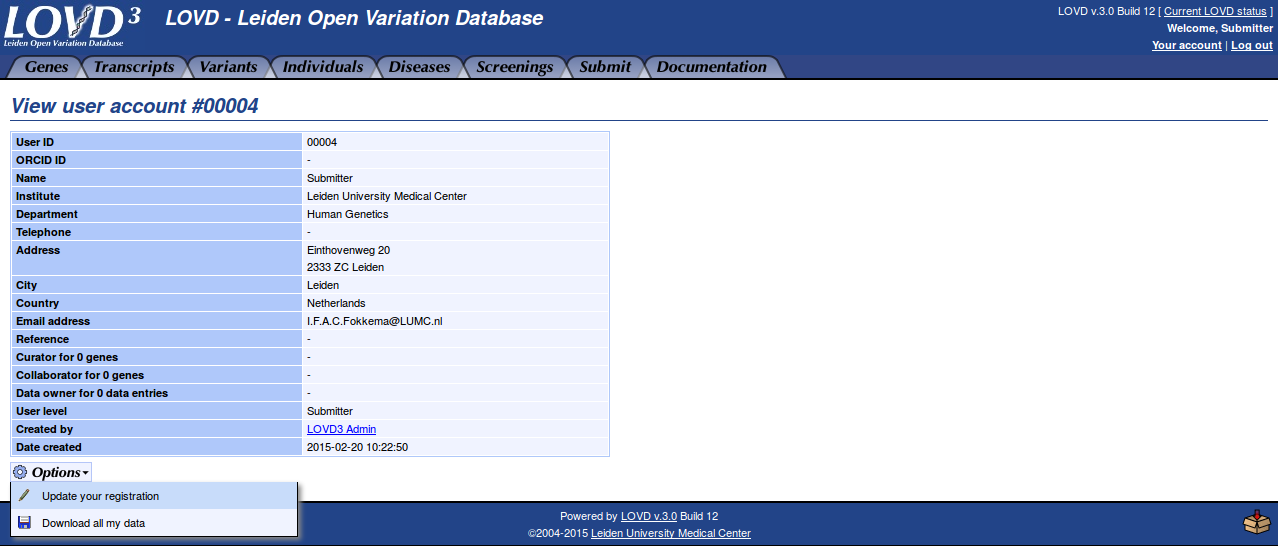
\includegraphics[width=\linewidth]
		   	 {/curate_gene/submission_I.png}};
		  	\begin{scope}[x={(image.south east)},y={(image.north west)}]
		      \draw[red,ultra thick,rounded corners] (0.895,0.9) rectangle (0.965,0.93);
					\draw[<-, >=latex, \pointercolor, line width=\pointerwidth] (0.895,0.9125) to node[black]{A} (0.795,0.9125);
		      \draw[red,ultra thick,rounded corners] (0.005,0.07) rectangle (0.15,0.12);
					\draw[<-, >=latex, \pointercolor, line width=\pointerwidth] (0.15,0.095) to node[black]{B} (0.25,0.095);
					%\drawgrid %help grid when positioning the boxes and pointers
		  	\end{scope}
			\end{tikzpicture}}
	  \caption{To change the users registration information, click on the ``Your account'' link (A).
	   Click the Options drop down menu and select ``Update your registration''.}
		\label{fig:submission_I}
  \end{shaded}
\end{figure}

\begin{figure}[ht]
  \begin{shaded}
		\frame{
			\begin{tikzpicture}
		  	\node[anchor=south west,inner sep=0] (image) at (0,0) {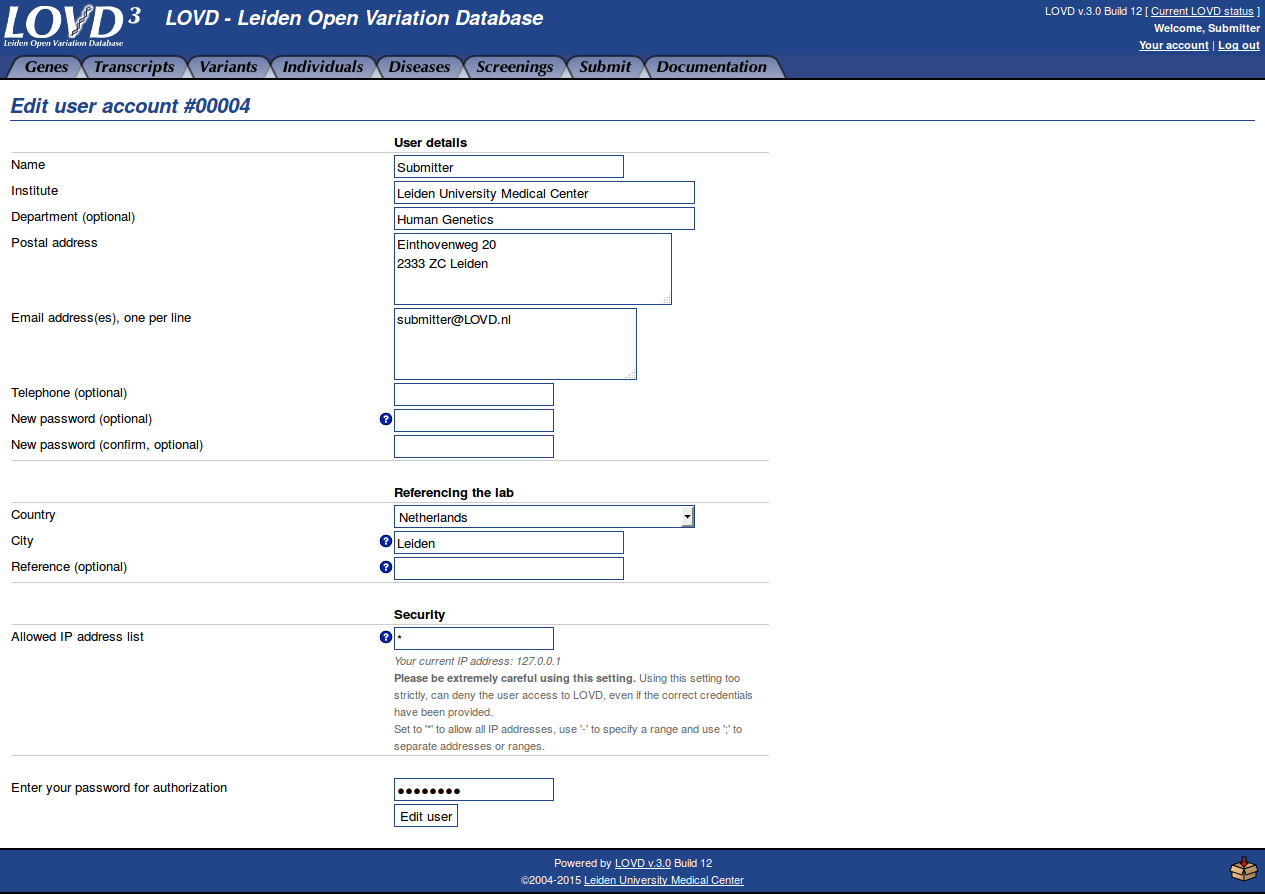
\includegraphics[width=\linewidth]
		   	 {/curate_gene/submission_II.png}};
		  	\begin{scope}[x={(image.south east)},y={(image.north west)}]
		      %\draw[red,ultra thick,rounded corners] (0.025,0.37) rectangle (0.1,0.405);
					%\draw[<-, >=latex, \pointercolor, line width=\pointerwidth] (0.1,0.3875) to node[black]{A} (0.2,0.3875);
					%\drawgrid %help grid when positioning the boxes and pointers
		  	\end{scope}
			\end{tikzpicture}}
	  \caption{Change the e-mail address to your e-mail address in the same way as you have done 
	   in figure \ref{fig:edit_curator_IV}}
		\label{fig:submission_II}
  \end{shaded}
\end{figure}

\begin{figure}[ht]
  \begin{shaded}
		\frame{
			\begin{tikzpicture}
		  	\node[anchor=south west,inner sep=0] (image) at (0,0) {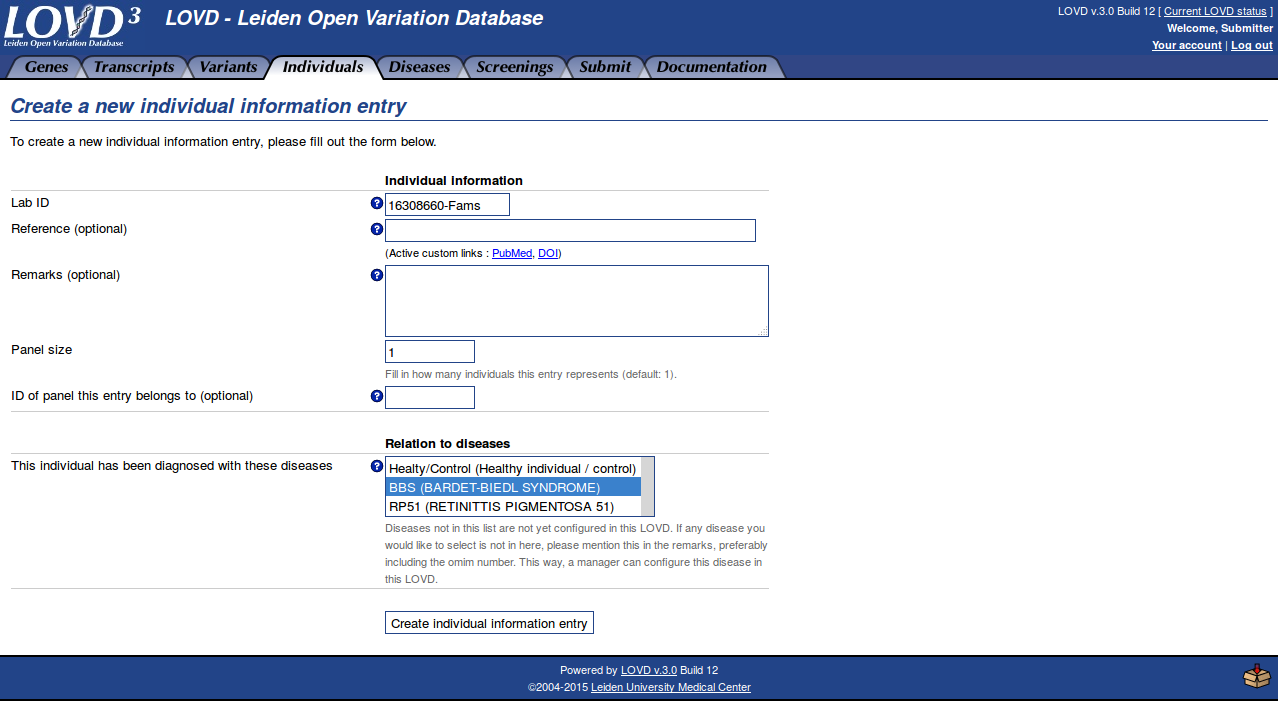
\includegraphics[width=\linewidth]
		   	 {/curate_gene/submission_III.png}};
		  	\begin{scope}[x={(image.south east)},y={(image.north west)}]
		      \draw[red,ultra thick,rounded corners] (0.44,0.875) rectangle (0.51,0.93);
					\draw[<-, >=latex, \pointercolor, line width=\pointerwidth] (0.51,0.9025) to node[black]{A} (0.61,0.9025);
		      \draw[red,ultra thick,rounded corners] (0.285,0.685) rectangle (0.415,0.755);
					\draw[<-, >=latex, \pointercolor, line width=\pointerwidth] (0.415,0.72) to node[black]{B} (0.515,0.72);
		      \draw[red,ultra thick,rounded corners] (0.285,0.255) rectangle (0.52,0.38);
					\draw[<-, >=latex, \pointercolor, line width=\pointerwidth] (0.52,0.3175) to node[black]{C} (0.62,0.3175);
					%\drawgrid %help grid when positioning the boxes and pointers
		  	\end{scope}
			\end{tikzpicture}}
	  \caption{When you are logged in as a submitter, 
	   a submission starts with creating new individual information.\newline
	  Click on the Submit menu tab (A).
	  Enter the Lab ID (B) and select a related disease (C).
	  Provide more information when available.\newline
	  When you are done, click ``Create individual information entry''.}
		\label{fig:submission_III}
  \end{shaded}
\end{figure}

\begin{figure}[ht]
  \begin{shaded}
		\frame{
			\begin{tikzpicture}
		  	\node[anchor=south west,inner sep=0] (image) at (0,0) {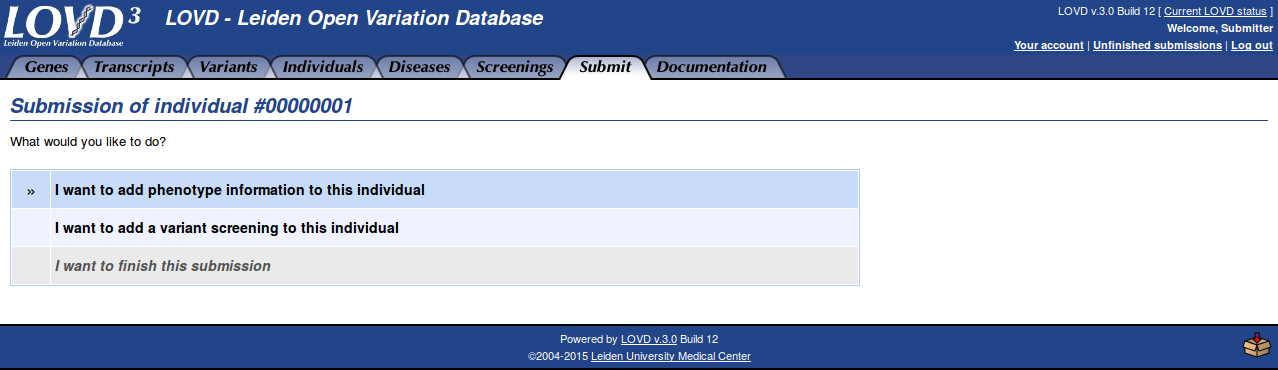
\includegraphics[width=\linewidth]
		   	 {/curate_gene/submission_IV.png}};
		  	\begin{scope}[x={(image.south east)},y={(image.north west)}]
		      \draw[red,ultra thick,rounded corners] (0.025,0.435) rectangle (0.4,0.55);
					\draw[<-, >=latex, \pointercolor, line width=\pointerwidth] (0.4,0.4925) to node[black]{A} (0.5,0.4925);
		      \draw[red,ultra thick,rounded corners] (0.85,0.85) rectangle (0.96,0.9);
					\draw[<-, >=latex, \pointercolor, line width=\pointerwidth] (0.85,0.875) to node[black]{B} (0.75,0.875);
					%\drawgrid %help grid when positioning the boxes and pointers
		  	\end{scope}
			\end{tikzpicture}}
	  \caption{To add phenotype information to the individual you just created, click ``I want to add phenotype
	   information to this individual'' (A).\newline
	   Note that during a submission you can not return to the individual information entry form in case you made an
	    error or forgot something. 
	   If you made an error or forgot something, you have to proceed with your submission and when ready you can edit
	    your individual via the ``Unfinished submissions'' link (B). 
	   This also applies for phenotypes, screenings and variants.}
		\label{fig:submission_IV}
  \end{shaded}
\end{figure}

\begin{figure}[ht]
  \begin{shaded}
		\frame{
			\begin{tikzpicture}
		  	\node[anchor=south west,inner sep=0] (image) at (0,0) {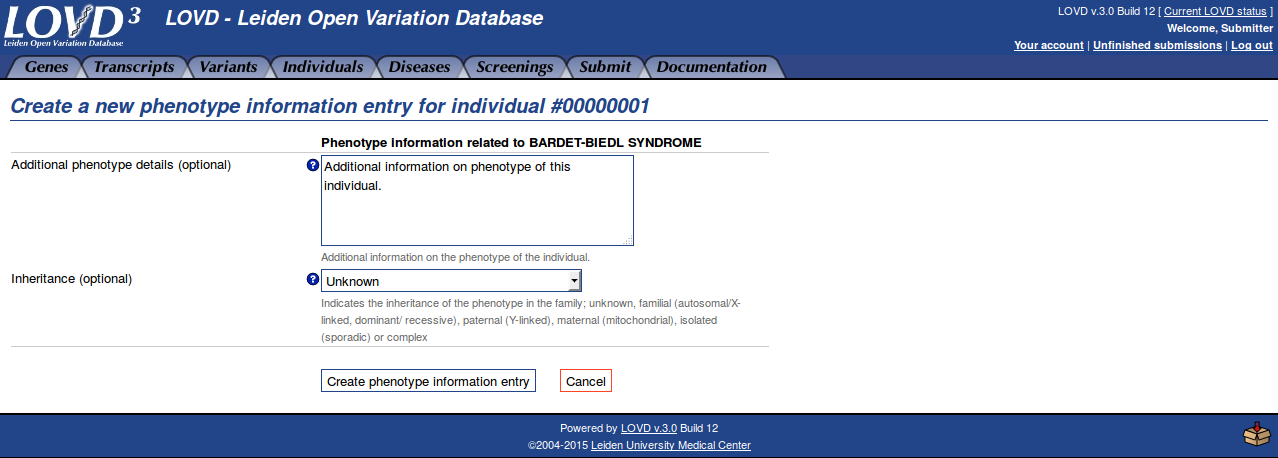
\includegraphics[width=\linewidth]
		   	 {/curate_gene/submission_V.png}};
		  	\begin{scope}[x={(image.south east)},y={(image.north west)}]
		      %\draw[red,ultra thick,rounded corners] (0.235,0.45) rectangle (0.555,0.71);
					%\draw[<-, >=latex, \pointercolor, line width=\pointerwidth] (0.555,0.58) to node[black]{} (0.655,0.58);
					%\drawgrid %help grid when positioning the boxes and pointers
		  	\end{scope}
			\end{tikzpicture}}
	  \caption{Enter any additional phenotype information you may have, and when ready click ``Create phenotype information entry''.}
		\label{fig:submission_V}
  \end{shaded}
\end{figure}

\begin{figure}[ht]
  \begin{shaded}
		\frame{
			\begin{tikzpicture}
		  	\node[anchor=south west,inner sep=0] (image) at (0,0) {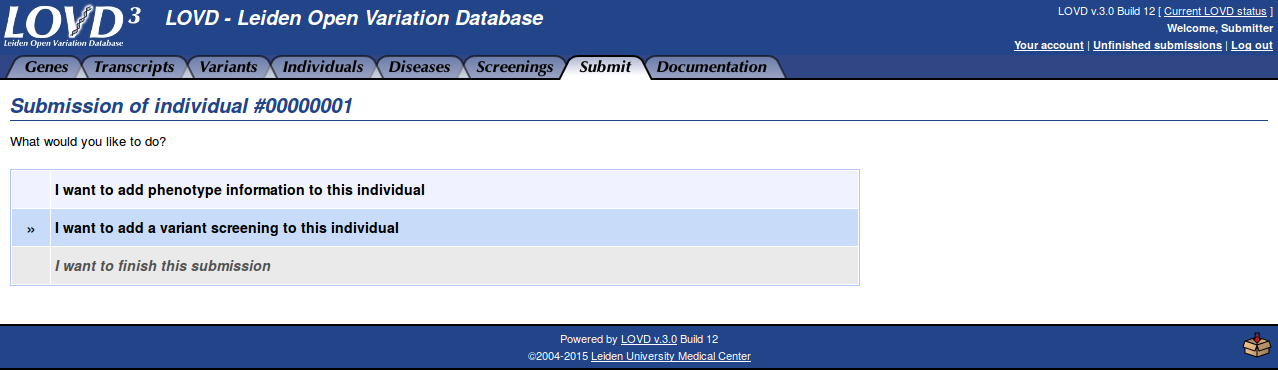
\includegraphics[width=\linewidth]
		   	 {/curate_gene/submission_VI.png}};
		  	\begin{scope}[x={(image.south east)},y={(image.north west)}]
		      %\draw[red,ultra thick,rounded corners] (0.025,0.345) rectangle (0.4,0.435);
					%\draw[<-, >=latex, \pointercolor, line width=\pointerwidth] (0.4,0.39) to node[black]{} (0.5,0.39);
		      %\drawgrid %help grid when positioning the boxes and pointers
		  	\end{scope}
			\end{tikzpicture}}
	  \caption{To add a variant screening, click ``I want to add a variant screening to this individual''.}
		\label{fig:submission_VI}
  \end{shaded}
\end{figure}

\begin{figure}[ht]
  \begin{shaded}
		\frame{
			\begin{tikzpicture}
		  	\node[anchor=south west,inner sep=0] (image) at (0,0) {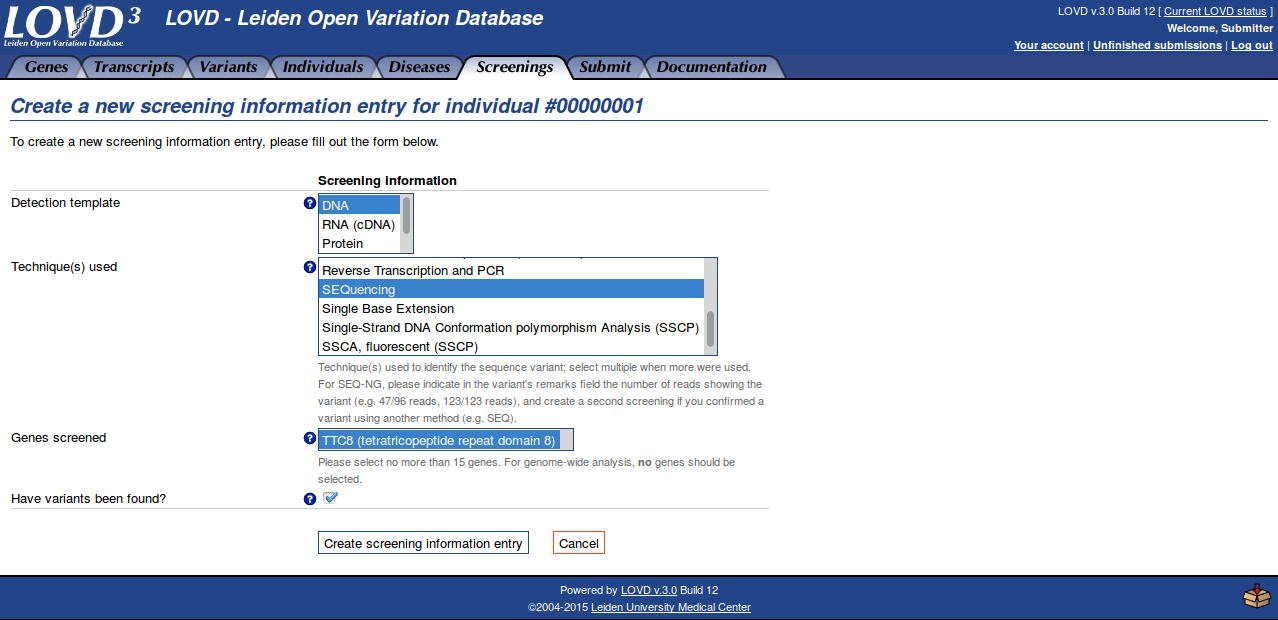
\includegraphics[width=\linewidth]
		   	 {/curate_gene/submission_VII.png}};
		  	\begin{scope}[x={(image.south east)},y={(image.north west)}]
		      \draw[red,ultra thick,rounded corners] (0.23,0.65) rectangle (0.33,0.69);
					\draw[<-, >=latex, \pointercolor, line width=\pointerwidth] (0.33,0.67) to node[black]{A} (0.43,0.67);
		      \draw[red,ultra thick,rounded corners] (0.23,0.52) rectangle (0.56,0.555);
					\draw[<-, >=latex, \pointercolor, line width=\pointerwidth] (0.56,0.5375) to node[black]{B} (0.66,0.5375);
		      \draw[red,ultra thick,rounded corners] (0.23,0.27) rectangle (0.46,0.31);
					\draw[<-, >=latex, \pointercolor, line width=\pointerwidth] (0.46,0.29) to node[black]{C} (0.56,0.29);
					%\drawgrid %help grid when positioning the boxes and pointers
		  	\end{scope}
			\end{tikzpicture}}
	  \caption{Select a detection template (A), technique(s) used (B) and gene(s) screened (C). 
	  Multiple lines can be selected in all three fields.\newline
	  When you made your selection, click ``Create screening information entry''.}
		\label{fig:submission_VII}
  \end{shaded}
\end{figure}

\begin{figure}[ht]
  \begin{shaded}
		\frame{
			\begin{tikzpicture}
		  	\node[anchor=south west,inner sep=0] (image) at (0,0) {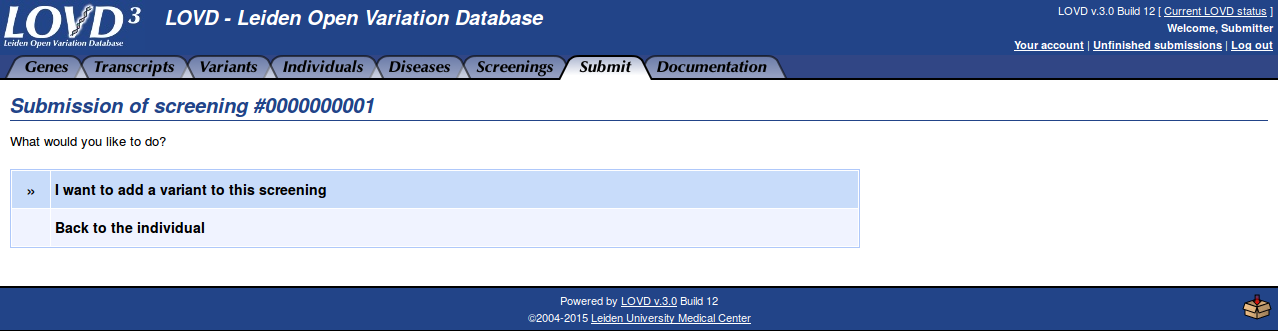
\includegraphics[width=\linewidth]
		   	 {/curate_gene/submission_VIII.png}};
		  	\begin{scope}[x={(image.south east)},y={(image.north west)}]
		      %\draw[red,ultra thick,rounded corners] (0.025,0.37) rectangle (0.3,0.495);
					%\draw[<-, >=latex, \pointercolor, line width=\pointerwidth] (0.3,0.4325) to node[black]{A} (0.4,0.4325);
					%\drawgrid %help grid when positioning the boxes and pointers
		  	\end{scope}
			\end{tikzpicture}}
	  \caption{Now we're going to add a variant to the screening we just entered. 
	  Click ``I want to add a variant to this screening''.}
		\label{fig:submission_VIII}
  \end{shaded}
\end{figure}

\begin{figure}[ht]
  \begin{shaded}
		\frame{
			\begin{tikzpicture}
		  	\node[anchor=south west,inner sep=0] (image) at (0,0) {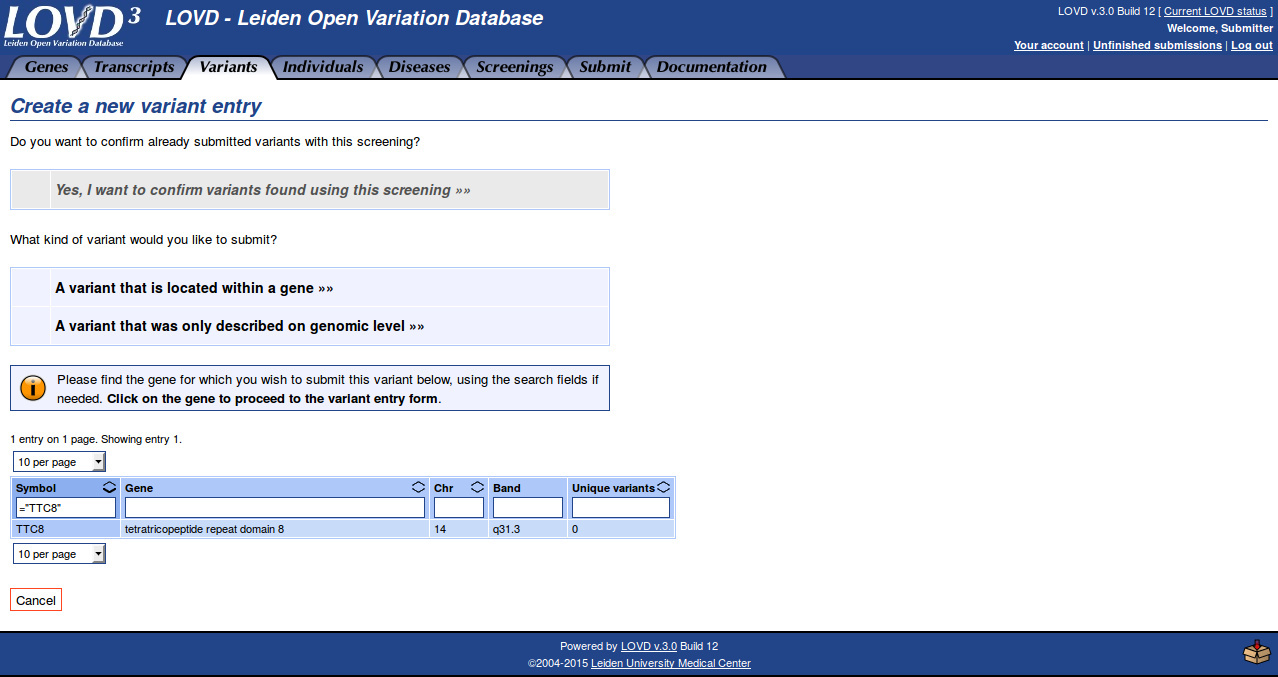
\includegraphics[width=\linewidth]
		   	 {/curate_gene/submission_IX.png}};
		  	\begin{scope}[x={(image.south east)},y={(image.north west)}]
		      \draw[red,ultra thick,rounded corners] (0.025,0.55) rectangle (0.3,0.6);
					\draw[<-, >=latex, \pointercolor, line width=\pointerwidth] (0.3,0.575) to node[black]{A} (0.4,0.575);
		      \draw[red,ultra thick,rounded corners] (0.01,0.2) rectangle (0.3,0.24);
					\draw[<-, >=latex, \pointercolor, line width=\pointerwidth] (0.3,0.22) to node[black]{B} (0.4,0.22);
					%\drawgrid %help grid when positioning the boxes and pointers
		  	\end{scope}
			\end{tikzpicture}}
	  \caption{Click ``A variant that is located within a gene'' (A).
	  Thereafter, you can select a gene to which you want to add a variant. Click on TTC8 (B). }
		\label{fig:submission_IX}
  \end{shaded}
\end{figure}

\begin{figure}[ht]
  \begin{shaded}
		\frame{
			\begin{tikzpicture}
		  	\node[anchor=south west,inner sep=0] (image) at (0,0) {\includegraphics[width=\linewidth]
		   	 {/curate_gene/submission_X.png}};
		  	\begin{scope}[x={(image.south east)},y={(image.north west)}]
		      \draw[red,ultra thick,rounded corners] (0.29,0.752) rectangle (0.6,0.786);
					\draw[<-, >=latex, \pointercolor, line width=\pointerwidth] (0.6,0.769) to node[black]{} (0.7,0.769);
					%\drawgrid %help grid when positioning the boxes and pointers
		  	\end{scope}
			\end{tikzpicture}}
	  \caption{In chapter ``\nameref{edit_columns_legends}'' we have changed the order and the legend of custom column 
	   ``Published\_as''. 
	  The position of the ``Published\_as'' field depends on what you have changed there.\newline
	  Move your mouse over the blue help icon in front of the ``Published as'' field, 
	   to see the changes you made in the description or notes fields.\newline
	 	Enter ``c.284A>G'' in the DNA change field of transcript NM\_144596.2 and click ``Map to genome''.}
		\label{fig:submission_X}
  \end{shaded}
\end{figure}

\begin{figure}[ht]
  \begin{shaded}
		\frame{
			\begin{tikzpicture}
		  	\node[anchor=south west,inner sep=0] (image) at (0,0) {\includegraphics[width=\linewidth]
		   	 {/curate_gene/submission_XI.png}};
		  	\begin{scope}[x={(image.south east)},y={(image.north west)}]
		      \draw[red,ultra thick,rounded corners] (0.29,0.7) rectangle (0.52,0.76);
					\draw[<-, >=latex, \pointercolor, line width=\pointerwidth] (0.52,0.73) to node[black]{A} (0.62,0.73);
		      \draw[red,ultra thick,rounded corners] (0.29,0.47) rectangle (0.52,0.55);
					\draw[<-, >=latex, \pointercolor, line width=\pointerwidth] (0.52,0.51) to node[black]{B} (0.62,0.51);
		      \draw[red,ultra thick,rounded corners] (0.29,0.23) rectangle (0.52,0.26);
					\draw[<-, >=latex, \pointercolor, line width=\pointerwidth] (0.52,0.245) to node[black]{C} (0.62,0.245);
					%\drawgrid %help grid when positioning the boxes and pointers
		  	\end{scope}
			\end{tikzpicture}}
	  \caption{The fields at arrows A, B and C are filled by LOVD.}
		\label{fig:submission_XI}
  \end{shaded}
\end{figure}

\begin{figure}[ht]
  \begin{shaded}
		\frame{
			\begin{tikzpicture}
		  	\node[anchor=south west,inner sep=0] (image) at (0,0) {\includegraphics[width=\linewidth]
		   	 {/curate_gene/submission_XII.png}};
		  	\begin{scope}[x={(image.south east)},y={(image.north west)}]
		      \draw[red,ultra thick,rounded corners] (0.29,0.78) rectangle (0.37,0.81);
		      \draw[red,ultra thick,rounded corners] (0.29,0.675) rectangle (0.515,0.71);
		      \draw[red,ultra thick,rounded corners] (0.29,0.615) rectangle (0.515,0.65);
		      \draw[red,ultra thick,rounded corners] (0.29,0.545) rectangle (0.37,0.575);
		      \draw[red,ultra thick,rounded corners] (0.29,0.38) rectangle (0.515,0.41);
		      \draw[red,ultra thick,rounded corners] (0.29,0.168) rectangle (0.61,0.215);
					\draw[<-, >=latex, \pointercolor, line width=\pointerwidth] (0.61,0.1915) to node[black]{A} (0.71,0.1915);
		      \draw[red,ultra thick,rounded corners] (0.29,0.11) rectangle (0.515,0.164);
					%\drawgrid %help grid when positioning the boxes and pointers
		  	\end{scope}
			\end{tikzpicture}}
	  \caption{Fill in the other fields as indicated in the figure. 
	  Below the reference field, the active custom links are displayed (A).\newline
	  When you hover your mouse cursor over the active custom links, 
	  you will see a small window with some custom link information and examples.\newline
	  When you click on one of the active custom links, the custom link format is entered in the field.}
		\label{fig:submission_XII}
  \end{shaded}
\end{figure}

\begin{figure}[ht]
  \begin{shaded}
		\frame{
			\begin{tikzpicture}
		  	\node[anchor=south west,inner sep=0] (image) at (0,0) {\includegraphics[width=\linewidth]
		   	 {/curate_gene/submission_XIII.png}};
		  	\begin{scope}[x={(image.south east)},y={(image.north west)}]
		      %\draw[red,ultra thick,rounded corners] (0.025,0.24) rectangle (0.23,0.33);
					%\draw[<-, >=latex, \pointercolor, line width=\pointerwidth] (0.23,0.285) to node[black]{} (0.33,0.285);
					%\drawgrid %help grid when positioning the boxes and pointers
		  	\end{scope}
			\end{tikzpicture}}
	  \caption{You can finish your submission by clicking ``I want to finish this submission''.
	  Check your e-mail, you should have received a message that there is a new submission in your gene database.}
		\label{fig:submission_XIII}
  \end{shaded}
\end{figure}










\chapter{Curating a submission}
The objective of this chapter is:
\begin{enumerate}
	\item 
	Curate submitted data.
\end{enumerate}
To start this chapter:
\begin{itemize}
	\item
	Log in as Curator (username: curator, password: curator1).
\end{itemize}
\begin{figure}[ht]
  \begin{shaded}
		\frame{
			\begin{tikzpicture}
		  	\node[anchor=south west,inner sep=0] (image) at (0,0) {\includegraphics[width=\linewidth]
		   	 {/curate_gene/curate_IA.png}};
		  	\begin{scope}[x={(image.south east)},y={(image.north west)}]
		      \draw[red,ultra thick,rounded corners] (0.01,0.6) rectangle (0.1,0.7);
					\draw[<-, >=latex, \pointercolor, line width=\pointerwidth] (0.1,0.65) to node[black]{A} (0.2,0.65);
		      \draw[red,ultra thick,rounded corners] (0.22,0.62) rectangle (0.6,0.72);
					\draw[<-, >=latex, \pointercolor, line width=\pointerwidth] (0.6,0.67) to node[black]{B} (0.7,0.67);
					%\drawgrid %help grid when positioning the boxes and pointers
		  	\end{scope}
			\end{tikzpicture}}
	  \caption{
	  Click on the Configuration menu tab.
	  On the left part of your screen you can see an overview of the number of variants in your gene database (A).
	  One variant in uncurated.
	  To curate the new variant, click the ``View all uncurated variant entries in the TTC8 gene database'' 
		 link listed under	``Curating TTC8 variants''(B).\newline
		Note: the link in the submission email that was send to the curator will take you directly to the following page. }
		\label{fig:curate_IA}
  \end{shaded}
\end{figure}

\begin{figure}[ht]
  \begin{shaded}
		\frame{
			\begin{tikzpicture}
		  	\node[anchor=south west,inner sep=0] (image) at (0,0) {\includegraphics[width=\linewidth]
		   	 {/curate_gene/curate_IB.png}};
		  	\begin{scope}[x={(image.south east)},y={(image.north west)}]
		      %\draw[red,ultra thick,rounded corners] (0.09,0.75) rectangle (0.15,0.84);
					%\draw[<-, >=latex, \pointercolor, line width=\pointerwidth] (0.15,0.795) to node[black]{A} (0.25,0.795);
		      %\draw[red,ultra thick,rounded corners] (0.01,0.25) rectangle (0.7,0.3);
					%\draw[<-, >=latex, \pointercolor, line width=\pointerwidth] (0.7,0.275) to node[black]{} (0.8,0.275);
					%\drawgrid %help grid when positioning the boxes and pointers
		  	\end{scope}
			\end{tikzpicture}}
	  \caption{
	  You will see a variant which is grey and with status pending, click on the variant.}
		\label{fig:curate_IB}
  \end{shaded}
\end{figure}

\begin{figure}[ht]
  \begin{shaded}
		\frame{
			\begin{tikzpicture}
		  	\node[anchor=south west,inner sep=0] (image) at (0,0) {\includegraphics[width=\linewidth]
		   	 {/curate_gene/curate_II.png}};
		  	\begin{scope}[x={(image.south east)},y={(image.north west)}]
		      \draw[red,ultra thick,rounded corners] (0.32,0.835) rectangle (0.41,0.86);
					\draw[<-, >=latex, \pointercolor, line width=\pointerwidth] (0.41,0.8475) to node[black]{A} (0.51,0.8475);
		      \draw[red,ultra thick,rounded corners] (0.32,0.635) rectangle (0.38,0.66);
					\draw[<-, >=latex, \pointercolor, line width=\pointerwidth] (0.38,0.6475) to node[black]{B} (0.48,0.6475);
		      \draw[red,ultra thick,rounded corners] (0.005,0.495) rectangle (0.2,0.525);
					\draw[<-, >=latex, \pointercolor, line width=\pointerwidth] (0.2,0.51) to node[black]{C} (0.3,0.51);
					%\drawgrid %help grid when positioning the boxes and pointers
		  	\end{scope}
			\end{tikzpicture}}
	  \caption{On the ``View genomic variant'' page you can see that the individual (A) and the variant (B) both have 
	   status pending.\newline
	  If the information is correct, you can curate the variant (C) by clicking on the Options drop down menu and
	   selecting ``Publish (curate) variant entry''. 
	  This variant is now published and visible to others.}
		\label{fig:curate_II}
  \end{shaded}
\end{figure}

\begin{figure}[ht]
  \begin{shaded}
		\frame{
			\begin{tikzpicture}
		  	\node[anchor=south west,inner sep=0] (image) at (0,0) {\includegraphics[width=\linewidth]
		   	 {/curate_gene/curate_III.png}};
		  	\begin{scope}[x={(image.south east)},y={(image.north west)}]
		      \draw[red,ultra thick,rounded corners] (0.32,0.81) rectangle (0.41,0.832);
					\draw[<-, >=latex, \pointercolor, line width=\pointerwidth] (0.41,0.821) to node[black]{B} (0.51,0.821);
		      \draw[red,ultra thick,rounded corners] (0.32,0.57) rectangle (0.38,0.59);
					\draw[<-, >=latex, \pointercolor, line width=\pointerwidth] (0.38,0.58) to node[black]{A} (0.48,0.58);
					%\drawgrid %help grid when positioning the boxes and pointers
		  	\end{scope}
			\end{tikzpicture}}
	  \caption{The variant status is now public (A).
	  To publish the individual data, click on the individual ID link (B)}
		\label{fig:curate_III}
  \end{shaded}
\end{figure}


\begin{figure}[ht]
  \begin{shaded}
		\frame{
			\begin{tikzpicture}
		  	\node[anchor=south west,inner sep=0] (image) at (0,0) {\includegraphics[width=\linewidth]
		   	 {/curate_gene/curate_IV.png}};
		  	\begin{scope}[x={(image.south east)},y={(image.north west)}]
		      \draw[red,ultra thick,rounded corners] (0.005,0.555) rectangle (0.12,0.59);
					\draw[<-, >=latex, \pointercolor, line width=\pointerwidth] (0.12,0.5725) to node[black]{A} (0.22,0.5725);
					%\drawgrid %help grid when positioning the boxes and pointers
		  	\end{scope}
			\end{tikzpicture}}
	  \caption{If the information is correct, you can curate the individual (A) by clicking on the Options drop down menu
	   and selecting ``Publish (curate) individual entry''. }
		\label{fig:curate_IV}
  \end{shaded}
\end{figure}

\begin{figure}[ht]
  \begin{shaded}
		\frame{
			\begin{tikzpicture}
		  	\node[anchor=south west,inner sep=0] (image) at (0,0) {\includegraphics[width=\linewidth]
		   	 {/curate_gene/curate_V.png}};
		  	\begin{scope}[x={(image.south east)},y={(image.north west)}]
		      \draw[red,ultra thick,rounded corners] (0.005,0.455) rectangle (0.42,0.495);
					\draw[<-, >=latex, \pointercolor, line width=\pointerwidth] (0.42,0.475) to node[black]{A} (0.52,0.475);
					%\drawgrid %help grid when positioning the boxes and pointers
		  	\end{scope}
			\end{tikzpicture}}
	  \caption{The phenotype submission is still gray. 
	  Click on the phenotype entry to curate.}
		\label{fig:curate_V}
  \end{shaded}
\end{figure}

\begin{figure}[ht]
  \begin{shaded}
		\frame{
			\begin{tikzpicture}
		  	\node[anchor=south west,inner sep=0] (image) at (0,0) {\includegraphics[width=\linewidth]
		   	 {/curate_gene/curate_VI.png}};
		  	\begin{scope}[x={(image.south east)},y={(image.north west)}]
		      %\draw[red,ultra thick,rounded corners] (0.005,0.08) rectangle (0.19,0.15);
					%\draw[<-, >=latex, \pointercolor, line width=\pointerwidth] (0.19,0.115) to node[black]{} (0.29,0.115);
					%\drawgrid %help grid when positioning the boxes and pointers
		  	\end{scope}
			\end{tikzpicture}}
	  \caption{If the information is correct, you can curate the phenotype by clicking on the Options drop down menu
	   and select ``Publish (curate) phenotype entry''. }
		\label{fig:curate_VI}
  \end{shaded}
\end{figure}









\chapter{Export and import}
The objectives of this chapter are:
\begin{enumerate}
	\item 
	Export your gene data
	\item 
	Delete your gene data
	\item
	Import your gene data
\end{enumerate}
To start this chapter:
\begin{itemize}
	\item
	Log in as Curator (username: curator password: curator1).
\end{itemize}

\begin{figure}[ht]
  \begin{shaded}
		\frame{
			\begin{tikzpicture}
		  	\node[anchor=south west,inner sep=0] (image) at (0,0) {\includegraphics[width=\linewidth]
		   	 {/curate_gene/export_I.png}};
		  	\begin{scope}[x={(image.south east)},y={(image.north west)}]
		      \draw[red,ultra thick,rounded corners] (0.61,0.34) rectangle (0.89,0.44);
					\draw[<-, >=latex, \pointercolor, line width=\pointerwidth] (0.89,0.39) to node[black]{} (0.99,0.39);
					%\drawgrid %help grid when positioning the boxes and pointers
		  	\end{scope}
			\end{tikzpicture}}
	  \caption{On two places you can download your gene related data.
	  You can do that from the Configuration area, 
	   by clicking the ``Download all data from the TTC8 gene database'' link listed under ``Download gene, 
	   transcript, variant and individual data''.
	  Or you can do that from the ``View gene'' page, see figure \ref{fig:export_II}. }
		\label{fig:export_I}
  \end{shaded}
\end{figure}

\begin{figure}[ht]
  \begin{shaded}
		\frame{
			\begin{tikzpicture}
		  	\node[anchor=south west,inner sep=0] (image) at (0,0) {\includegraphics[width=\linewidth]
		   	 {/curate_gene/export_II.png}};
		  	\begin{scope}[x={(image.south east)},y={(image.north west)}]
		      \draw[red,ultra thick,rounded corners] (0.005,0.145) rectangle (0.18,0.165);
					\draw[<-, >=latex, \pointercolor, line width=\pointerwidth] (0.18,0.155) to node[black]{A} (0.28,0.155);
		      \draw[red,ultra thick,rounded corners] (0.005,0.24) rectangle (0.18,0.26);
					\draw[<-, >=latex, \pointercolor, line width=\pointerwidth] (0.18,0.25) to node[black]{B} (0.28,0.25);
					%\drawgrid %help grid when positioning the boxes and pointers
		  	\end{scope}
			\end{tikzpicture}}
	  \caption{Also from the ``View gene'' page you can download the gene related data. 
	  Click the Options drop down menu and select ``Download all this gene's data'' (A).
	  The download begins immediately.\newline
	  When you have downloaded and saved your gene data, we are going to empty this gene database.
	  Click the Options drop down menu and select ``Empty this gene database'' (B).}
		\label{fig:export_II}
  \end{shaded}
\end{figure}

\begin{figure}[ht]
  \begin{shaded}
		\frame{
			\begin{tikzpicture}
		  	\node[anchor=south west,inner sep=0] (image) at (0,0) {\includegraphics[width=\linewidth]
		   	 {/curate_gene/export_IV.png}};
		  	\begin{scope}[x={(image.south east)},y={(image.north west)}]
					%\drawgrid %help grid when positioning the boxes and pointers
		  	\end{scope}
			\end{tikzpicture}}
	  \caption{You get an extra warning that you are about to delete data and which data.
	  Note that genes, transcripts and diseases are not deleted.
	  Confirm with your password.}
		\label{fig:export_IV}
  \end{shaded}
\end{figure}

\begin{figure}[ht]
  \begin{shaded}
		\frame{
			\begin{tikzpicture}
		  	\node[anchor=south west,inner sep=0] (image) at (0,0) {\includegraphics[width=\linewidth]
		   	 {/curate_gene/export_V.png}};
		  	\begin{scope}[x={(image.south east)},y={(image.north west)}]
		      \draw[red,ultra thick,rounded corners] (0.215,0.19) rectangle (0.6,0.24);
					\draw[<-, >=latex, \pointercolor, line width=\pointerwidth] (0.6,0.215) to node[black]{} (0.7,0.215);
					%\drawgrid %help grid when positioning the boxes and pointers
		  	\end{scope}
			\end{tikzpicture}}
	  \caption{Only managers can import data into LOVD3 for the moment. 
		Therefore log in as Manager (username: manager, password: manager1).
	  You can import the data from the Setup area.
	  Click the ``Import data using the LOVD import format'' link listed under ``Download \& Import''.}
		\label{fig:export_V}
  \end{shaded}
\end{figure}

\begin{figure}[ht]
  \begin{shaded}
		\frame{
			\begin{tikzpicture}
		  	\node[anchor=south west,inner sep=0] (image) at (0,0) {\includegraphics[width=\linewidth]
		   	 {/curate_gene/export_VII.png}};
		  	\begin{scope}[x={(image.south east)},y={(image.north west)}]
		      \draw[red,ultra thick,rounded corners] (0.235,0.44) rectangle (0.6,0.56);
					\draw[<-, >=latex, \pointercolor, line width=\pointerwidth] (0.6,0.5) to node[black]{A} (0.7,0.5);
		      \draw[red,ultra thick,rounded corners] (0.235,0.145) rectangle (0.3,0.18);
					\draw[<-, >=latex, \pointercolor, line width=\pointerwidth] (0.3,0.1625) to node[black]{B} (0.4,0.1625);
					%\drawgrid %help grid when positioning the boxes and pointers
		  	\end{scope}
			\end{tikzpicture}}
	  \caption{Select the file you downloaded at the beginning of this chapter (A).
	  Check the Simulate check box to do a test import.
	  Click ``Import file''.}
		\label{fig:export_VII}
  \end{shaded}
\end{figure}

\begin{figure}[ht]
  \begin{shaded}
		\frame{
			\begin{tikzpicture}
		  	\node[anchor=south west,inner sep=0] (image) at (0,0) {\includegraphics[width=\linewidth]
		   	 {/curate_gene/export_VIII.png}};
		  	\begin{scope}[x={(image.south east)},y={(image.north west)}]
		      \draw[red,ultra thick,rounded corners] (0.005,0.51) rectangle (0.85,0.59);
					\draw[<-, >=latex, \pointercolor, line width=\pointerwidth] (0.85,0.55) to node[black]{A} (0.95,0.55);
		      \draw[red,ultra thick,rounded corners] (0.235,0.38) rectangle (0.6,0.49);
					\draw[<-, >=latex, \pointercolor, line width=\pointerwidth] (0.6,0.435) to node[black]{B} (0.7,0.435);
		      \draw[red,ultra thick,rounded corners] (0.235,0.125) rectangle (0.3,0.155);
					\draw[<-, >=latex, \pointercolor, line width=\pointerwidth] (0.3,0.14) to node[black]{C} (0.4,0.14);
					%\drawgrid %help grid when positioning the boxes and pointers
		  	\end{scope}
			\end{tikzpicture}}
	  \caption{The import simulation has been successful (A). 
		But a warning is given, this is because the diseases were not deleted. 
		LOVD recognized the disease in the import file.\newline
		To do a real import, select the file again (B), uncheck the Simulate check box (C) and click ``Import file''.}
		\label{fig:export_VIII}
  \end{shaded}
\end{figure}

\begin{figure}[ht]
  \begin{shaded}
		\frame{
			\begin{tikzpicture}
		  	\node[anchor=south west,inner sep=0] (image) at (0,0) {\includegraphics[width=\linewidth]
		   	 {/curate_gene/export_IX.png}};
		  	\begin{scope}[x={(image.south east)},y={(image.north west)}]
					%\drawgrid %help grid when positioning the boxes and pointers
		  	\end{scope}
			\end{tikzpicture}}
	  \caption{Import is done}
		\label{fig:export_IX}
  \end{shaded}
\end{figure}

\begin{figure}[ht]
  \begin{shaded}
		\frame{
			\begin{tikzpicture}
		  	\node[anchor=south west,inner sep=0] (image) at (0,0) {\includegraphics[width=\linewidth]
		   	 {/curate_gene/export_X.png}};
		  	\begin{scope}[x={(image.south east)},y={(image.north west)}]
		      \draw[red,ultra thick,rounded corners] (0.32,0.83) rectangle (0.4,0.85);
					\draw[<-, >=latex, \pointercolor, line width=\pointerwidth] (0.4,0.84) to node[black]{} (0.5,0.84);
		      \draw[red,ultra thick,rounded corners] (0.005,0.09) rectangle (0.1,0.12);
					\draw[<-, >=latex, \pointercolor, line width=\pointerwidth] (0.1,0.105) to node[black]{} (0.2,0.105);
					%\drawgrid %help grid when positioning the boxes and pointers
		  	\end{scope}
			\end{tikzpicture}}
	  \caption{Your database now looks the same as before you deleted the gene's data.
	  Only the ID's are different: individual ID, screening ID and variant ID.}
		\label{fig:export_X}
  \end{shaded}
\end{figure}



\chapter{Example E-mails}
\section{Welcome new submitter}

Dear \ldots,
\vskip1em

First of all, welcome as new submitter to the gene variant database at the Leiden Muscular Dystrophy pages 	
 (www.DMD.nl);
great that you have started to actually submit gene variants!
\vskip1em

In future new entries will become uploaded automatically and without notification, 
 unless we have specific questions.
Please note that after login you can update your records when more information comes in. 
When you notice mistakes or omissions in the other entries of the database, 
	please do not forget to notify us immediately.
\vskip1em

Regarding your submissions we have some questions -just to be sure that we curate them correctly;

\noindent\ldots
\vskip1em

Since this is the first variant(s) you report we assume that you may have found more in the past. 
If so, please note that the database tries to store ALL variants identified and not only variants that have 
 not been reported before. 
This includes ALL variant found in a specific patient (pathogenic AND non-pathogenic). 
When you have identified more gene variants, please consider submitting these as well.
Note that for submission of larger sets of variants we can help you: 
you send us the variants in electronic format, preferably a spreadsheet format. 
\vskip1em

\noindent Yours sincerely, 
\vskip1em

Curator: \ldots

Department: \ldots

Institute:  \ldots

Database URL:  \ldots

\clearpage
\section{New publication}

Dear \ldots,
\vskip1em

In PubMed we came across your article entitled ``\ldots'' (\ldots).
When the final version of the paper is out, we would very much appreciate to receive a copy of the paper, 
 preferably in electronic format (.PDF).
\vskip1em

We have added the sequence variants described to the DMD gene variant database at
\newline (http://www.LOVD.nl/DMD).
Please have a look to see whether we have done this correctly.
We concluded that some patients were described earlier by \ldots et al; is this correct?
Some details from the paper were not clear (seebelow), please check and clarify;
\begin{description}
	\item 
	\ldots one variant was described as \ldots but this seems not correct \ldots
	\item
	\ldots it was unclear which variants where found in which combinations (recessive disease)
	\item
	\ldots you list some variants as percentages but we would appreciate to list the number of variants alleles / 
	 alleles tested (like 12/98)
	 \item
	 \ldots phenotype data are largely lacking, we would appreciate to receive any details you may have
\end{description}
\vskip1em
In the mean time you probably have identified more variants in the gene and/or other genes involved in the 
 neuromuscular disorders covered by our databases.
We would very much appreciate to receive an overview of these variants to be able to add them to the database.
Note that the database tries to store ALL variants identified and not only variants that have not been 
 reported before. 
This includes ALL variants found in a specific patient (pathogenic AND non-pathogenic). 
When you have identified more gene variants, please consider to submit these as well. 
Note that for submission of larger sets of variants we can offer our help when you send us the variants in  
 electronic format, preferably a spreadsheet format. 
\vskip1em

We noticed that you mention our database in your paper. 
Please consider to register as submitter and submit all variants you identify directly to the database. 
Note that only a complete and fully up-to-date database is most helpful for those using it, 
 in particular those using it to perform accurate DNA diagnostics for patients and their relatives.
\vskip1em

\noindent Yours sincerely, 
\vskip1em

Curator: \ldots

Department: \ldots

Institute:  \ldots

Database URL:  \ldots




\end{document}

%10
\chapter{}
%5
\section{}
%3
\subsection{}
%1
\subsubsection{}


%%%%%%%%%%%%%%%%%%%%%%%%%%%%%%%%%%%%%%%%%% NEW MAXIMUM LINE LENGTH (120 char) %%%%%%%%%%%%%%%%%%%%%%%%%%%%%%%%%%%%%%%%%%
